%Version 3.1 December 2024
% See section 11 of the User Manual for version history
%
%%%%%%%%%%%%%%%%%%%%%%%%%%%%%%%%%%%%%%%%%%%%%%%%%%%%%%%%%%%%%%%%%%%%%%
%%                                                                 %%
%% Please do not use \input{...} to include other tex files.       %%
%% Submit your LaTeX manuscript as one .tex document.              %%
%%                                                                 %%
%% All additional figures and files should be attached             %%
%% separately and not embedded in the \TeX\ document itself.       %%
%%                                                                 %%
%%%%%%%%%%%%%%%%%%%%%%%%%%%%%%%%%%%%%%%%%%%%%%%%%%%%%%%%%%%%%%%%%%%%%

%%\documentclass[referee,sn-basic]{sn-jnl}% referee option is meant for double line spacing

%%=======================================================%%
%% to print line numbers in the margin use lineno option %%
%%=======================================================%%

%%\documentclass[lineno,pdflatex,sn-basic]{sn-jnl}% Basic Springer Nature Reference Style/Chemistry Reference Style

%%=========================================================================================%%
%% the documentclass is set to pdflatex as default. You can delete it if not appropriate.  %%
%%=========================================================================================%%

%%\documentclass[sn-basic]{sn-jnl}% Basic Springer Nature Reference Style/Chemistry Reference Style

%%Note: the following reference styles support Namedate and Numbered referencing. By default the style follows the most common style. To switch between the options you can add or remove �Numbered� in the optional parenthesis. 
%%The option is available for: sn-basic.bst, sn-chicago.bst%  
 
%%\documentclass[pdflatex,sn-nature]{sn-jnl}% Style for submissions to Nature Portfolio journals
%%\documentclass[pdflatex,sn-basic]{sn-jnl}% Basic Springer Nature Reference Style/Chemistry Reference Style
%%\documentclass[pdflatex,sn-mathphys-num]{sn-jnl}% Math and Physical Sciences Numbered Reference Style
\documentclass[pdflatex,sn-mathphys-ay]{sn-jnl}% Math and Physical Sciences Author Year Reference Style
%%\documentclass[pdflatex,sn-aps]{sn-jnl}% American Physical Society (APS) Reference Style
%%\documentclass[pdflatex,sn-vancouver-num]{sn-jnl}% Vancouver Numbered Reference Style
%%\documentclass[pdflatex,sn-vancouver-ay]{sn-jnl}% Vancouver Author Year Reference Style
%%\documentclass[pdflatex,sn-apa]{sn-jnl}% APA Reference Style
%%\documentclass[pdflatex,sn-chicago]{sn-jnl}% Chicago-based Humanities Reference Style

%%%% Standard Packages
%%<additional latex packages if required can be included here>
\usepackage{nicefrac}
\usepackage{array}

\usepackage{graphicx}%
\usepackage{multirow}%
\usepackage{amsmath,amssymb,amsfonts}%
\usepackage{amsthm}%
\usepackage{mathrsfs}%
\usepackage[title]{appendix}%
\usepackage{xcolor}%
\usepackage{textcomp}%
\usepackage{manyfoot}%
\usepackage{booktabs}%
\usepackage{algorithm}%
\usepackage{algorithmicx}%
\usepackage{algpseudocode}%
\usepackage{listings}%
%%%%

%%%%%=============================================================================%%%%
%%%%  Remarks: This template is provided to aid authors with the preparation
%%%%  of original research articles intended for submission to journals published 
%%%%  by Springer Nature. The guidance has been prepared in partnership with 
%%%%  production teams to conform to Springer Nature technical requirements. 
%%%%  Editorial and presentation requirements differ among journal portfolios and 
%%%%  research disciplines. You may find sections in this template are irrelevant 
%%%%  to your work and are empowered to omit any such section if allowed by the 
%%%%  journal you intend to submit to. The submission guidelines and policies 
%%%%  of the journal take precedence. A detailed User Manual is available in the 
%%%%  template package for technical guidance.
%%%%%=============================================================================%%%%

%% as per the requirement new theorem styles can be included as shown below
\theoremstyle{thmstyleone}%
\newtheorem{theorem}{Theorem}%  meant for continuous numbers
%%\newtheorem{theorem}{Theorem}[section]% meant for sectionwise numbers
%% optional argument [theorem] produces theorem numbering sequence instead of independent numbers for Proposition
\newtheorem{proposition}[theorem]{Proposition}% 
%%\newtheorem{proposition}{Proposition}% to get separate numbers for theorem and proposition etc.

\theoremstyle{thmstyletwo}%
\newtheorem{example}{Example}%
\newtheorem{remark}{Remark}%

\theoremstyle{thmstylethree}%
\newtheorem{definition}{Definition}%

\raggedbottom
%%\unnumbered% uncomment this for unnumbered level heads

\begin{document}

\title[Planar equivalent layers for potential fields: 2. Geophysical implications and applications]{Planar equivalent layers for potential fields: 2. Geophysical implications and applications}

%%=============================================================%%
%% GivenName	-> \fnm{Joergen W.}
%% Particle	-> \spfx{van der} -> surname prefix
%% FamilyName	-> \sur{Ploeg}
%% Suffix	-> \sfx{IV}
%% \author*[1,2]{\fnm{Joergen W.} \spfx{van der} \sur{Ploeg} 
%%  \sfx{IV}}\email{iauthor@gmail.com}
%%=============================================================%%

\author*[1]{\fnm{Vanderlei C.} \sur{Oliveira Jr.}}\email{vanderlei@on.br}
\author[2]{\fnm{Christian} \sur{Gerhards}}\email{Christian.Gerhards@geophysik.tu-freiberg.de}
\author[1]{\fnm{Val{\' e}ria C. F.} \sur{Barbosa}}\email{valcris@on.br}
\author[1]{\fnm{Andr{\' e} L. A.} \sur{Reis}}\email{reisandreluis@on.br}
\author[1]{\fnm{Edson F.} \sur{Luza}}\email{edsonluza@on.br}
\author[2]{\fnm{Xinpeng} \sur{Huang}}\email{Xinpeng.huang@geophysik.tu-freiberg.de }


%\equalcont{These authors contributed equally to this work.}

\affil[1]{\orgdiv{Coordena{\c c}{\~ a}o de Geof{\' i}sica}, \orgname{Observat{\' o}rio Nacional}, \orgaddress{\street{General Jos{\' e} Cristino st.}, \city{Rio de Janeiro}, \country{Brazil}}}

\affil[2]{\orgdiv{Institute of Geophysics and Geoinformatics}, \orgname{TU Bergakademie Freiberg}, \orgaddress{\street{Gustav-Zeuner-Str.}, \city{Freiberg}, \country{Germany}}}

%%==================================%%
%% Sample for unstructured abstract %%
%%==================================%%

\abstract{The equivalent-layer technique has been widely applied in geophysics since the 1960s 
for potential-field transformations as well as for processing and interpreting 
gravity and magnetic data. Despite its success, the method has traditionally relied 
on empirical assumptions, with limited attention to its theoretical foundation. In a 
companion paper, we have established a rigorous theoretical framework for planar equivalent layers. 
Here, we examine the implications of these theoretical results for the empirical 
approaches commonly used in the geophysical literature. Through 
numerical experiments, we demonstrate the numerical consistency and close agreement between the 
closed-form expressions for planar equivalent layers and the discrete layers obtained 
by linear inversion of potential-field data. Our results confirm that multiple planar equivalent 
layers can be employed to achieve the same potential-field transformations.}

%%================================%%
%% Sample for structured abstract %%
%%================================%%

% \abstract{\textbf{Purpose:} The abstract serves both as a general introduction to the topic and as a brief, non-technical summary of the main results and their implications. The abstract must not include subheadings (unless expressly permitted in the journal's Instructions to Authors), equations or citations. As a guide the abstract should not exceed 200 words. Most journals do not set a hard limit however authors are advised to check the author instructions for the journal they are submitting to.
% 
% \textbf{Methods:} The abstract serves both as a general introduction to the topic and as a brief, non-technical summary of the main results and their implications. The abstract must not include subheadings (unless expressly permitted in the journal's Instructions to Authors), equations or citations. As a guide the abstract should not exceed 200 words. Most journals do not set a hard limit however authors are advised to check the author instructions for the journal they are submitting to.
% 
% \textbf{Results:} The abstract serves both as a general introduction to the topic and as a brief, non-technical summary of the main results and their implications. The abstract must not include subheadings (unless expressly permitted in the journal's Instructions to Authors), equations or citations. As a guide the abstract should not exceed 200 words. Most journals do not set a hard limit however authors are advised to check the author instructions for the journal they are submitting to.
% 
% \textbf{Conclusion:} The abstract serves both as a general introduction to the topic and as a brief, non-technical summary of the main results and their implications. The abstract must not include subheadings (unless expressly permitted in the journal's Instructions to Authors), equations or citations. As a guide the abstract should not exceed 200 words. Most journals do not set a hard limit however authors are advised to check the author instructions for the journal they are submitting to.}

\keywords{potential theory, geophysics, potential-field methods, equivalent-layer technique}

%%\pacs[JEL Classification]{D8, H51}

%%\pacs[MSC Classification]{35A01, 65L10, 65L12, 65L20, 65L70}

\maketitle

\section{Introduction}

The equivalent-layer technique has long being used in applied geophysics for 
for processing and interpreting potential-field data. 
It consists in approximating a discrete set of potential-field data 
by a linear combination of harmonic functions representing the potential field 
due to a discrete set of virtual sources (e.g., monopoles, dipoles, prisms).
These virtual sources are called \textit{equivalent sources} and are commonly disposed on a surface 
forming a discrete \textit{equivalent layer}, which is ``equivalent" 
in the sense that it satisfactorily reproduces the observed potential-field data.
The general approach involves estimating the constant physical property of the equivalent sources 
(e.g., density, mass, isotropic magnetic susceptibility, magnetization intensity, magnetic moment intensity) 
by numerically solving a constrained linear inverse problem.
The technique can be used to accomplish various data processing steps, such as interpolation, 
upward (or downward) continuation, gradient data processing, merging multiple data sets, 
estimating density models from gravity data, 
computing the amplitude of the anomalous magnetic field, 
transforming total-field anomalies into field components, 
as well as estimating the magnetization direction and computing the reduction to the pole
of magnetic data. 
Further details on the equivalent-layer technique can be found in the recent review by 
\citet{oliveirajr_etal2023}.

Most of methods based on the equivalent-layer technique 
are based on the widely accepted \textit{equivalent-layer principle}, which 
refers to the empirical generalizations by which most of the studies found in the geophysical literature justify 
the existence of equivalent layers allowing computing potential-field transformations.
In the companion paper ``Planar equivalent layers for potential fields: Part 1 -- Theoretical insights'',
we have proposed a comprehensive theoretical framework with the purpose of replacing the 
equivalent-layer principle with the \textit{planar equivalent-layer theorem}, 
which guarantees the existence of continuous and planar equivalent layers 
that reproduce the gravitational and magnetic induction fields due to 3D sources, 
even for the case in which the layer crosses them. 
From our theoretical developments, we have deduced different closed-form expressions for continuous and planar 
equivalent layers that are defined on the same horizontal surface to reproduce the a given potential-field data.

Here, we use the theoretical framework presented in the companion paper
``Planar equivalent layers for potential fields: Part 1 -- Theoretical insights" to explain 
well-established empirical approaches commonly found in the geophysical literature about the 
equivalent-layer technique, such as joint processing of gravity-gradient data 
\cite[e.g.,][]{barnes_lumley2011}, conversion of gravity disturbance data into the 
gravity-gradient tensor \cite[e.g.,][]{piauilino_etal2019_seg, oliveirajr_etal2023} and the use 
dipole layers to reduce magnetic data to the pole 
\citep[e.g.,][]{emilia1973, bhattacharyya_chan1977, silva1986, leao-silva_1989, oliveirajr_etal2013, 
li_etal2014, oliveirajr_etal2015, ribeiro_filho_etal2020, reis_etal2020, li-etal2021, takahashi-etal2022, piauilino_etal2025}. 
Results obtained from numerical simulations show that the estimated discrete equivalent layers 
commonly used in practical applications approximate the closed-form expressions we have presented in the 
companion paper. We also illustrate the application of an alternative equivalent-layer of dipoles to 
interpret airborne magnetic data over a complex alkaline province in central part of Brazil. Our results show that
the alternative approach can bring valuable information on the horizontal position of the true sources without 
imposing any information on their total-magnetization direction.

\section{Theoretical background}

Consider a of 3D gravity or magnetic sources be defined over a closed region 
$\overline{\mathcal{V}'}$ located in the subsurface, with top limited by a vertical 
coordinate $z^{t}_{0}$ in a topocentric Cartesian coordinate system with axes 
$x$, $y$, and $z$ pointing to north, east and down, respectively.
The potential field produced by the 3D sources at observation points 
$\mathbf{r} = (x, y, z)^{\top}$ (Fig.  \ref{fig:Figure1}) is represented by:
\begin{equation}
	d^{o}(\mathbf{r}) = D_{d} \, U(\mathbf{r}) \: , 
	\quad \mathbf{r} \notin \overline{\mathcal{V}'} \: ,
	\label{eq:observed-data-space}
\end{equation}
where $D_{d}$ is a space-domain differential operator acting on the Newtonian potential
\begin{equation}
	U(\mathbf{r}) = \kappa \iiint\limits_{\overline{\mathcal{V}'}}
	\sigma(\mathbf{r}') \: \frac{1}{\| \mathbf{r} - \mathbf{r}'\|}
	\: d\mathcal{V}' \: , 
	\quad \mathbf{r} \notin \overline{\mathcal{V}'} \: ,
	\label{eq:potential-U-space}
\end{equation}
$\kappa$ is a proportionality constant,
$\tfrac{1}{\| \mathbf{r} - \mathbf{r}' \|}$ is the inverse distance function
between the observation point $\mathbf{r}$ and a point 
$\mathbf{r}' = (x', y', z')^{\top} \in \overline{\mathcal{V}'}$
and $\sigma$ is the scalar function representing 
the density (contrast) or total-magnetization intensity within the sources.
\cite{oliveirajr_etal2026_1} propose the following general formula to define the 
space-domain differential operator $D_{d}$ (Eq. \ref{eq:observed-data-space}) 
and its corresponding counterpart $\alpha_{d}$ in the Fourier domain:
\begin{equation}
	D(\ell, \hat{\mathbf{u}}) = 
	\left( \hat{\mathbf{u}}^{\top} \nabla \right)^{\ell} \Leftrightarrow
	\alpha(\ell, \hat{\mathbf{u}}) = \left( \hat{\mathbf{u}}^{\top} \mathbf{k} \right)^{\ell} \: ,
	\quad \ell \in \{ 0, 1, 2 \} \: ,
	\label{eq:diff-operators-generic}
\end{equation}
where $\hat{\mathbf{u}}$ is a constant unit vector,
$\nabla$ is the vector differential operator nabla, 
$\mathbf{k} = ( \mathtt{i} \, k_{x} \, , \, \mathtt{i} \, k_{y} \, , \, k)^{\top}$
\cite{pedersen1978}, $k_{x}$ and $k_{y}$ and represent the wavenumbers along the $x$ and $y$
directions and $k = \sqrt{k_{x}^{2} + k_{y}^{2}}$.
Different potential fields $d^{o}$ (Eq. \ref{eq:observed-data-space}) can be 
defined by properly setting $\ell$ and $\hat{\mathbf{u}}$ in the left side of equation
\ref{eq:diff-operators-generic}. 

Many geophysical applications require computing potential-field transformations that convert the
observed potential field $d^{o}$ (Eq. \ref{eq:observed-data-space}) into another potential field 
given by
\begin{equation}
	f(\mathbf{r}) = D_{f} U(\mathbf{r}) \: , 
	\quad \mathbf{r} \notin \overline{\mathcal{V}'} \: ,
	\label{eq:transformed-field-space}
\end{equation}
where $D_{f}$ is a space-domain differential operator 
(Eq. \ref{eq:diff-operators-generic}) acting on $U$ (Eq. \ref{eq:potential-U-space}).
The ``equivalent-layer technique'' is the common approach to compute potential-field transformations
in the space domain and this is usually performed in two steps.
The first consists in estimating a ``continuous equivalent layer'' $p_{\varepsilon}$ 
\cite{oliveirajr_etal2026_1} over a horizontal surface $\mathcal{S}''$ with constant vertical
coordinate $z''_{0}$, so that the predicted potential field
\begin{equation}
	d_{\varepsilon}(\mathbf{r})
	= \int\limits_{-\infty}^{\infty}\int\limits_{-\infty}^{\infty}
	p_{\varepsilon}(\mathbf{r}'') \, D_{a} \Psi(\mathbf{r}, \mathbf{r}'') \:\: d\mathcal{S}''
	\: , \quad z < z''_{0} \: ,
	\label{eq:predicted-data-continuous-layer}
\end{equation}
satisfactorily approximates the observed potential field $d^{o}$ 
(Eq. \ref{eq:observed-data-space}) within a predefined error level,
where $D_{a}$ is a space-domain differential operator 
(Eq. \ref{eq:diff-operators-generic}) acting on the scaled inverse 
distance function between $\mathbf{r}$ and 
$\mathbf{r}'' = (x'', y'', z''_{0})^{\top} \in \mathcal{S}''$ given by
\begin{equation}
	\Psi(\mathbf{r}, \mathbf{r}'') = 
	\frac{1}{2\pi} \: 
	\frac{1}{\| \mathbf{r} - \mathbf{r}'' \|} \: , 
	\quad \mathbf{r} \ne \mathbf{r}'' \: .
	\label{eq:Psi}
\end{equation}
The second step in the equivalent-layer technique involves using the estimated $p_{\varepsilon}$ 
(Eq. \ref{eq:predicted-data-continuous-layer}) to compute the transformed potential field
\begin{equation}
	f_{\varepsilon}(\mathbf{r})
	= \int\limits_{-\infty}^{\infty}\int\limits_{-\infty}^{\infty}
	p_{\varepsilon}(\mathbf{r}'') \, D_{t}\Psi(\mathbf{r}, \mathbf{r}'') \:\: d\mathcal{S}'' 
	\: , \quad z < z''_{0} \: ,
	\label{eq:transformed-field-continuous-layer}
\end{equation}
where $D_{t}$ is a space-domain differential operator acting on the function 
$\Psi$ (Eq. \ref{eq:Psi}).
The underlying assumption in the equivalent-layer technique is that the transformed potential 
field $f_{\varepsilon}$ (Eq. \ref{eq:transformed-field-continuous-layer}) approximates 
the desired potential field $f$ (Eq. \ref{eq:transformed-field-space}).

The planar equivalent-layer theorem formulated and proved by \cite{oliveirajr_etal2026_1} 
guarantees the existence of equivalent layers $p_{\varepsilon}$ 
(Eq. \ref{eq:predicted-data-continuous-layer}), even 
if they are defined over a planar surface $\mathcal{S}''$ that intersects the true sources.
Those authors also proposed a general expression for $p_{\varepsilon}$ in the Fourier domain 
given by
\begin{equation}
	\mathcal{F} [ p_{\varepsilon}(\mathbf{r}'') ] =
	\tfrac{k \, \alpha_{d}}{\alpha_{a}} \,
	\mathcal{F} [ U_{\varepsilon}(\mathbf{r}'') ] \: ,
	\quad \mathbf{r}'' \in \mathcal{S}'' \: ,
	\label{eq:p-Fourier}
\end{equation}
where $\mathcal{F} [ \cdot ]$ denotes the two-dimensional Fourier transform computed 
with respect to the spatial coordinates $x$ and $y$, on 
the horizontal surface $\mathcal{S}''$ with constant vertical coordinate $z''_{0}$;
$\alpha_{d}$ and $\alpha_{a}$ are the corresponding Fourier-domain 
representation of the operators $D_{d}$ and $D_{a}$ (Eq(s). \ref{eq:observed-data-space}
and \ref{eq:predicted-data-continuous-layer}),
respectively; $k = \sqrt{k_{x}^{2} + k_{y}^{2}}$, where $k_{x}$ and $k_{y}$ represent the 
wavenumbers along the $x$ and $y$ directions, respectively; and $U_{\varepsilon}$ is an 
auxiliary potential that approximates $U$ (Eq. \ref{eq:potential-U-space}).
\cite{oliveirajr_etal2026_1} provided the following two possible expressions to define 
$U_{\varepsilon}$ in the Fourier domain:
\begin{equation}
	\mathcal{F} \left[ U_{\varepsilon}(\mathbf{r}'') \right] = 
	\begin{cases}
		\mathcal{F} \left[ U(\mathbf{r}^{\dagger}) \right] 
		e^{\, k \, (z''_{0} - z^{\dagger}_{0})} & , 
		\quad 0 < k \le k_{\varepsilon} \\
		0 & , \quad k > k_{\varepsilon} 
	\end{cases} \: ,
	\label{eq:potential-U-epsilon-Fourier-layer-1}
\end{equation}
where $k_{\varepsilon}$ is a fixed and possibly very large truncating wavenumber, and
\begin{equation}
	\mathcal{F} \left[ U_{\varepsilon}(\mathbf{r}'') \right] = 
	\tfrac{e^{\, k \, (z''_{0} - z^{\dagger}_{0})}}{1 + \mu_{\varepsilon} \, k^{2} \, e^{\, k \, (z''_{0} - z^{\dagger}_{0})}} \; 
	\mathcal{F} [ U(\mathbf{r}^{\dagger}) ] \: ,
	\label{eq:potential-U-epsilon-Fourier-layer-2}
\end{equation}
where $\mu_{\varepsilon}$ is a fixed positive regularization parameter imposing smoothness on 
$U$ according to \cite{pasteka_etal2012}. 
In Eq(s). \ref{eq:potential-U-epsilon-Fourier-layer-1} and 
\ref{eq:potential-U-epsilon-Fourier-layer-2},
$\mathbf{r}^{\dagger} = (x^{\dagger}, y^{\dagger}, z^{\dagger}_{0})^{\top}$ defines a point on 
a horizontal surface $\mathcal{S}^{\dagger}$ with constant vertical coordinate 
$z^{\dagger}_{0}$ located above the horizontal surface $\mathcal{S}''$, outside the sources, 
i.e., with $z^{\dagger}_{0} < z''_{0}$ and $z^{\dagger}_{0} < z^{t}_{0}$.

\cite{oliveirajr_etal2026_1} also show that the layer $p_{\varepsilon}$ leads to a transformed 
potential field $f_{\varepsilon}$ (Eq. \ref{eq:transformed-field-continuous-layer}) that 
is defined in the Fourier domain by 
\begin{equation}
	\mathcal{F} [ f_{\varepsilon}(\mathbf{r}^{\dagger}) ] =
	\mathcal{F} \left[ p_{\varepsilon}(\mathbf{r}'') \right]
	\alpha_{t} \, \mathcal{F} [ \Psi(\mathbf{r}^{\dagger}, \mathbf{r}'') ] \: , 
	\quad z^{\dagger}_{0} < z''_{0} \: ,
	\label{eq:transformed-field-continuous-layer-Fourier}
\end{equation}
where $\alpha_{t}$ is the Fourier representation of the operator $D_{t}$ (Eq. \ref{eq:transformed-field-continuous-layer}),
$\mathbf{r}^{\dagger} = (x^{\dagger}, y^{\dagger}, z^{\dagger}_{0})^{\top} \in \mathcal{S}^{\dagger}$,
$\mathbf{r}'' = (x'', y'', z''_{0})^{\top} \in \mathcal{S}''$ and
$\mathcal{F} [ \Psi(\mathbf{r}^{\dagger}, \mathbf{r}'') ] = \nicefrac{e^{-k \, (z''_{0} - z^{\dagger}_{0})}}{k}$ 
\citep[e.g.,][p. 275]{blakely1996} is the Fourier transform of $\Psi$ (Eq. \ref{eq:Psi}).
According to \cite{oliveirajr_etal2026_1}, the transformed potential field $f_{\varepsilon}$ defined in the Fourier
domain by Eq. \ref{eq:transformed-field-continuous-layer-Fourier} approximates $f$ 
(Eq. \ref{eq:transformed-field-space}) if
\begin{equation}
	\alpha_{t} = \left( \tfrac{\alpha_{a}}{\alpha_{d}} \right) \alpha_{f} \: ,
	\label{eq:alpha-t-generic}
\end{equation}
where $\alpha_{f}$ is the Fourier domain representation of the differential operator $D_{f}$ 
(Eq. \ref{eq:transformed-field-space}).

\begin{figure}
	\centering
	\noindent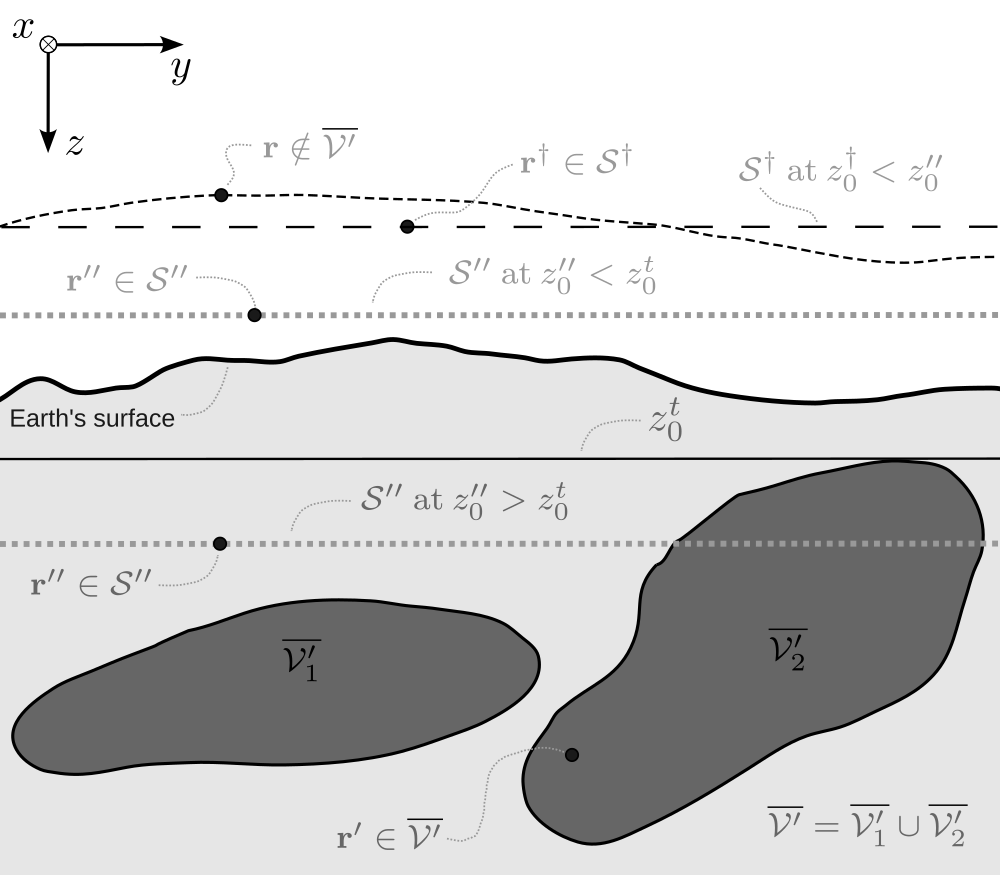
\includegraphics[width=0.8\textwidth]{figures/Figure2_1.png}
	\caption{%
		2D schematic representation of a vertical $yz$ plane crossing the sources (represented in dark gray),
		with $x$ axis pointing inward the page (represented by the ``$\otimes$" symbol).
		The sources are located in the subsurface (represented in light gray), over a 
		closed region $\overline{\mathcal{V}'}$ with top limited by the plane $z^{t}_{0}$. 
		The fine dashed lines represent two possible horizontal surfaces $\mathcal{S}''$, one located 
		at $z''_{0} < z^{t}_{0}$, above the sources, and another at $z''_{0} > z^{t}_{0}$, crossing the sources.
		The medium dashed line represents the surface containing the observation points 
		$\mathbf{r}$, all above $\mathcal{S}''$.
		The long dashed line represents a planar surface $\mathcal{S}^{\dagger}$ located 
		at $z^{\dagger}_{0} < z''_{0}$.
	}
	\label{fig:Figure1}
\end{figure}
\section{Geophysical implications}

\subsection{Equivalent layer vs. physical nature of the observed data}

The general expression proposed by \citeA{oliveirajr_etal2026} to define $p_{\varepsilon}$ in 
the Fourier domain (equation \ref{eq:p-Fourier}) allows setting different classes of 
equivalent layers.
In the particular case where $\alpha_{a} = \alpha_{d}$, for example, we obtain a Neumann's 
equivalent layer, which preserves the physical relationship between the observed data and the 
true sources. It means that, if the observed data correspond to the $y$-component of the 
magnetic induction field of the true sources, 
then the potential field predicted by the equivalent layer is also the $y$-component of the 
magnetic induction field of the equivalent sources. Most of the equivalent-layer methods use 
such layers to perform potential-field transformations.
On the other hand, layers $p_{\varepsilon}$ obtained with $\alpha_{a} \ne \alpha_{d}$ do not
preserve the physical relationship between the observed data and the true sources. 
This is the general case, for example, of layers obtained with $\alpha_{a} = k$, which are 
called Dirichlet's equivalent layers \cite{oliveirajr_etal2026}. Such layers are commonly used 
to perform the continuation of potential-field data. Obviously that Dirichlet's equivalent 
layers coincide with Neumann's equivalent layers for the particular case in which 
$\alpha_{d} = k$. 

One important aspect of equation \ref{eq:p-Fourier} is that it provides the theoretical 
foundation for common practices that have been empirically proved by several studies: 
equivalent layers are independent of the physical nature of the observed potential-field data 
and can be conveniently chosen according to the characteristics of the problem. Many authors 
have proposed equivalent-layer methods based on this empirical principle
\cite<e.g.,>[]{cordell1992, guspi_novara2009, li_etal2014, soler_uieda2021}, which is 
theoretically justified here for the first time by using the framework proposed by
\citeA{oliveirajr_etal2026}.

\subsection{Conversion of gravity disturbance into gravity-gradient data}

The common two-step approach to convert 
gravity disturbance data into the gravity-gradient tensor components
\cite<e.g.,>[]{piauilino_etal2019_seg, oliveirajr_etal2023} via equivalent-layer 
technique empirically presumes the existence of a single layer of 
monopoles that satisfactorily reproduces the gravitational potential and 
its derivatives of first and second orders, which are represented by the 
gravity disturbance and gravity-gradient data, respectively. 
Specifically, the first step in this approach consists in solving equation 
\ref{eq:predicted-data-continuous-layer} 
for $p_{\varepsilon}$ by using $D_{a} = \nicefrac{\partial}{\partial z}$, 
so that the predicted potential field $d_{\varepsilon}$ approximates the observed potential 
field $d^{o}$ (equation \ref{eq:observed-data-space}).
Then, in the second step, the estimated $p_{\varepsilon}$ is used to compute each 
gravity-gradient component with
equation \ref{eq:transformed-field-continuous-layer}, where $D_{t}$ is the corresponding 
differential operator associated with the gravity-gradient component.
For example, if the desired component is the $xy$, so 
$D_{t} = \nicefrac{\partial^{2}}{\partial x \, \partial y}$.

To understand why this approach works, let us first note that 
the differential operator associated with the observed gravity disturbance data (equation 
\ref{eq:observed-data-space}) is given by $D_{d} \equiv D(1, \hat{\mathbf{z}}) = 
\tfrac{\partial}{\partial z}$ in the space domain
or $\alpha_{d} \equiv \alpha(1, \hat{\mathbf{z}}) = k$ in the Fourier domain (equation 
\ref{eq:diff-operators-generic}),
where $\hat{\mathbf{z}} = (0, 0, 1)^{\top}$.
The first step consists in using $D_{a} = D_{d}$ in equation 
\ref{eq:predicted-data-continuous-layer} and 
estimating $p_{\varepsilon}$ so that the corresponding predicted potential field 
$d_{\varepsilon}$ approximates
the observed potential field $d^{o}$ (equation \ref{eq:observed-data-space}).
In this case, we conclude from equations \ref{eq:diff-operators-generic} and 
\ref{eq:p-Fourier} that $p_{\varepsilon}$ 
approximates the vertical derivative $\tfrac{\partial U}{\partial z}$ of $U$
(equation \ref{eq:potential-U-space}) on the surface $\mathcal{S}''$.

The second step to convert gravity disturbance data into gravity-gradient data involves using 
$p_{\varepsilon}$ to compute the gravity-gradient components, which are represented by the 
potential field $f$, with specific operators $D_{f}$ (equation 
\ref{eq:transformed-field-space}). 
Since our $p_{\varepsilon}$ (equation \ref{eq:p-Fourier}) is defined with $\alpha_{a} = 
\alpha_{d}$, it is a Neumann's equivalent layer \cite{oliveirajr_etal2026} and, consequently, 
any transformed potential field $f_{\varepsilon}$ 
(equation \ref{eq:transformed-field-continuous-layer}) must be defined with $D_{t} = D_{f}$, 
where $D_{f}$ is the space-domain 
operator associated with $f$ (equation \ref{eq:transformed-field-space}).
Consider, for example, that the desired potential field $f$ (equation 
\ref{eq:transformed-field-space}) is the gradient 
component $xy$. This component is defined by  
$D_{f} \equiv D(1, \hat{\mathbf{x}}) \, D(1, \hat{\mathbf{y}}) = \tfrac{\partial^{2}}{\partial x \, \partial y}$ in the
space domain, or 
$\alpha_{f} \equiv \alpha(1, \hat{\mathbf{x}}) \, \alpha(1, \hat{\mathbf{y}}) = \mathrm{i}^{2} \, k_{x} \, k_{y}$
in the Fourier domain (equation \ref{eq:diff-operators-generic}), where 
$\hat{\mathbf{x}} = (1, 0, 0)^{\top}$ and
$\hat{\mathbf{y}} = (0, 1, 0)^{\top}$.
In this case, the predicted $xy$ gradient component is obtained by evaluating 
$f_{\varepsilon}$ (equation \ref{eq:transformed-field-continuous-layer-Fourier}) with 
$D_{t} = \tfrac{\partial^{2}}{\partial x \, \partial y}$.
The remaining gradient components are evaluated in the same way, by using their corresponding 
operators $D_{f}$.

Thus, the common two-step approach to convert gravity disturbance into gravity
gradient data via equivalent-layer technique 
\cite<e.g.,>[]{piauilino_etal2019_seg, oliveirajr_etal2023} 
can be theoretically explained as an application of a particular Neumann's equivalent layer.

\subsection{Joint processing of gravity-gradient data}

Similarly to the previous approach to convert gravity disturbance data into gravity gradient 
data, the common approach to joint processing gravity gradient data 
\cite<e.g.,>[]{boggs-dransfield2004,barnes_lumley2011, martinez_li_2016} via equivalent-layer 
technique empirically presumes that a single equivalent layer $p_{\varepsilon}$ can be used to 
predict all gravity gradient components, i.e., that
\begin{equation}
	d^{uv}_{\varepsilon}(\mathbf{r}) = 
	\int\limits_{-\infty}^{\infty}\int\limits_{-\infty}^{\infty}
	p_{\varepsilon}(\mathbf{r}'') \, 
	\tfrac{\partial^{2} \Psi}{\partial u \, \partial v}(\mathbf{r}, \mathbf{r}'') \:\: 
	d\mathcal{S}'' \: , \quad z < z''_{0} \: ,
	\label{eq:gravity_gradient_layer}
\end{equation}
where $d^{uv}_{\varepsilon}$ approximates the gradient component $uv$, with 
$u, v \in \{x, y, z\}$.
This approach considers a set of equations defined by \ref{eq:gravity_gradient_layer}, each one
for a given gravity gradient component $uv$, and simultaneously solves then for the single 
layer $p_{\varepsilon}$.
Again, the existence of such layer can be deduced from equation \ref{eq:p-Fourier}, for the 
particular case in which 
$\alpha_{a} = \alpha_{d}$. In this case, $p_{\varepsilon}$ is a Neumann's equivalent layer 
\cite{oliveirajr_etal2026}.
Consider, for example, the gravity gradient component $xz$. In this case, 
the observed potential field is defined by 
$D_{d} \equiv D(1, \hat{\mathbf{x}}) \, D(1, \hat{\mathbf{z}}) = \tfrac{\partial^{2}}{\partial x \, \partial z}$ in the
space domain, or 
$\alpha_{d} \equiv \alpha(1, \hat{\mathbf{x}}) \, \alpha(1, \hat{\mathbf{z}}) = \mathrm{i} \, k_{x} \, k$
in the Fourier domain (equation \ref{eq:diff-operators-generic}), where 
$\hat{\mathbf{x}} = (1, 0, 0)^{\top}$ and
$\hat{\mathbf{y}} = (0, 0, 1)^{\top}$.
From equation \ref{eq:p-Fourier}, we conclude that the layer $p_{\varepsilon}$ obtained with 
$\alpha_{a} = \alpha_{d}$ represents the vertical derivative 
$\tfrac{\partial U_{\varepsilon}}{\partial z}$ of the auxiliary potential 
$U_{\varepsilon}$ (equations \ref{eq:potential-U-epsilon-Fourier-layer-1} and 
\ref{eq:potential-U-epsilon-Fourier-layer-2}) 
on the surface $\mathcal{S}''$.
The same conclusion is obtained for any other gravity gradient component defined with a 
different $uv$, which shows that there exists a single equivalent layer $p_{\varepsilon}$ that 
simultaneously fits all gravity gradient components.
We show here that the common approach to joint processing gravity gradient data 
\cite<e.g.,>[]{boggs-dransfield2004,barnes_lumley2011, martinez_li_2016} can be explained in 
terms of a Neumann's equivalent layer.

\subsection{The existence of a planar dipole layer}

A predominant trend in previous studies utilizing a planar equivalent layer of dipoles for 
magnetic-field transformations 
is to treat the layer as a purely mathematical abstraction employed for processing total-field 
anomaly data, a perspective exemplified by the remarks of \citeA{pedersen1989} concerning the 
research of \citeA{bhattacharyya_chan1977}.
Specifically, Pedersen pointed out that the first fundamental existence theorem for the 
Dirichlet's problem does not postulate that a general solution can be written as a layer of 
dipoles magnetized along its 
normal direction. In essence, Pedersen underscored that a dipole layer lacks physical 
significance.
In response, Chan affirmed that such a layer was employed in his work 
solely to address an integral equation, i.e., as a purely mathematical solution.

Since its inception in the 1960s, the equivalent-layer technique in applied geophysics has 
garnered relatively scant attention in terms of exploring the theoretical attributes of planar 
dipole layers capable of faithfully reproducing total-field anomaly data. 
This inquiry usually aims to discern the physical significance and possible link of such 
layers with boundary problems of potential theory.

Here, we leverage the theoretical framework proposed by \citeA{oliveirajr_etal2026} to infer 
within the purview of applied geophysics, for the first time, the existence of planar dipole 
layers capable of accurately and simultaneously reproducing the magnetic scalar potential and 
induction field components along any direction.
We first consider that the observed potential field $d^{o}$ (equation 
\ref{eq:observed-data-space}) is satisfactorily described by the differential operator 
$D_{d} \equiv D(1, \hat{\mathbf{u}}) \, D(1, \hat{\mathbf{v}})$
(equation \ref{eq:diff-operators-generic}), where $\hat{\mathbf{u}}$ defines the constant 
direction of the main geomagnetic field at the study area and $\hat{\mathbf{v}}$ the constant 
total-magnetization direction of the true magnetic sources.
From equation \ref{eq:diff-operators-generic}, we can show that 
(i) $D_{d} = \hat{\mathbf{u}}^{\top} \mathbf{H}_{U}(\mathbf{r}) \, \hat{\mathbf{v}}$,
where $\mathbf{H}_{U}$ is the Hessian matrix \cite<e.g.,>[p. 158]{kaplan2002} of
the potential $U$ (equation \ref{eq:potential-U-space}) and (ii) its corresponding 
Fourier domain representation is given by 
$\alpha_{d} = \left(\mathbf{k}^{\top} \hat{\mathbf{u}} \right)\left(\mathbf{k}^{\top} \hat{\mathbf{v}} \right)$.

The common equivalent-layer approach to process total-field anomaly data consists in 
estimating an equivalent layer $p_{\varepsilon}$ by solving the equation 
\ref{eq:predicted-data-continuous-layer},
with $D_{a} = \hat{\mathbf{u}}^{\top} \mathbf{H}_{\Psi}(\mathbf{r}) \, \hat{\mathbf{h}}$, 
where $\mathbf{H}_{\Psi}$ is the Hessian matrix \cite<e.g.,>[p. 158]{kaplan2002} of the 
function $\Psi$ (equation \ref{eq:Psi}) and $\hat{\mathbf{h}}$ is a constant unit vector not 
necessarily equal to $\hat{\mathbf{v}}$. From equation \ref{eq:diff-operators-generic}, we can 
show that the corresponding Fourier domain operator is given by 
$\alpha_{a} = \left(\mathbf{k}^{\top} \hat{\mathbf{u}} \right)\left(\mathbf{k}^{\top} \hat{\mathbf{h}} \right)$.
Then, by using the predefined $\alpha_{d}$ and $\alpha_{a}$ in equation \ref{eq:p-Fourier}, we 
obtain the following equivalent layer:
\begin{equation}
	\mathcal{F} [ p_{\varepsilon}(\mathbf{r}'') ] =
	k \, \tfrac{
		\left(\mathbf{k}^{\top} \hat{\mathbf{v}} \right)
		}{
		\left(\mathbf{k}^{\top} \hat{\mathbf{h}} \right)
		} \,
	\mathcal{F} \left[ U_{\varepsilon}(\mathbf{r}'') \right] \: .
	\label{eq:p-Fourier-dipoles}
\end{equation}

The particular equivalent layer given by equation \ref{eq:p-Fourier-dipoles} represents a 
planar layer of dipoles with constant magnetization direction $\hat{\mathbf{h}}$ and was 
deduced by considering
that $\hat{\mathbf{u}}$ is a unit vector having the same constant direction of the main 
geomagnetic field at the study area, i.e., by considering that the observed potential field is 
the approximated total-field anomaly \cite<e.g.,>[p. 179]{blakely1996}.
Let us now consider that the observed potential field data is a Cartesian component of the 
magnetic induction field. In this case, we can simply replace $\hat{\mathbf{u}}$ by the unit 
vector along the direction of 
magnetic induction field component. For example, if the observed potential field is the $x$ 
component of the magnetic induction field, then we have
(i) $D_{d} = \hat{\mathbf{x}}^{\top} \mathbf{H}_{U}(\mathbf{r}) \, \hat{\mathbf{v}}$, 
(ii) $\alpha_{d} = \left(\mathbf{k}^{\top} \hat{\mathbf{x}} \right)\left(\mathbf{k}^{\top} \hat{\mathbf{v}} \right)$,
(iii) $D_{a} = \hat{\mathbf{x}}^{\top} \mathbf{H}_{U}(\mathbf{r}) \, \hat{\mathbf{h}}$ and
(iv) $\alpha_{a} = \left(\mathbf{k}^{\top} \hat{\mathbf{x}} \right)\left(\mathbf{k}^{\top} \hat{\mathbf{h}} \right)$,
where $\hat{\mathbf{x}} = (1, 0, 0)^{\top}$. For the cases in which the observed potential field is the $y$ or 
$z$ component of the magnetic induction field, then we replace $\hat{\mathbf{x}}$ by the 
unit vector $\hat{\mathbf{y}} = (0, 1, 0)^{\top}$ or $\hat{\mathbf{z}} = (0, 0, 1)^{\top}$,
respectively. For these three Cartesian components of the magnetic induction field, we conclude from equation 
\ref{eq:p-Fourier} that the resultant equivalent layer is that defined by equation \ref{eq:p-Fourier-dipoles}.
It can also be easily verified that the same $p_{\varepsilon}$ given by equation 
\ref{eq:p-Fourier-dipoles} can be equally deduced if we consider that the 
observed potential field is the magnetic scalar potential. 
In this case, we have $\alpha_{d} = \left(\mathbf{k}^{\top} \hat{\mathbf{v}} \right)$ and 
$\alpha_{a} = \left(\mathbf{k}^{\top} \hat{\mathbf{h}} \right)$. 

The main conclusion obtained here is that a planar equivalent layer of dipoles $p_{\varepsilon}$ defined according 
to equation \ref{eq:p-Fourier-dipoles} simultaneously 
reproduces the magnetic scalar potential and any magnetic induction field component (including the approximated total-field anomaly) 
due to sources with constant total-magnetization direction defined by $\hat{\mathbf{v}}$, even if the layer has a constant magnetization 
direction defined by a unit vector $\hat{\mathbf{h}} \ne \hat{\mathbf{v}}$. 
This theoretical result explains, for example, why we can use a planar equivalent layer of dipoles with arbitrary constant 
magnetization direction $\hat{\mathbf{h}}$ to compute the magnetic induction field components or the amplitude of the 
magnetic induction field due to the true sources without presuming any information about the constant direction of their 
total magnetization \cite<e.g,>[]{li_etal_2021}.


\subsection{Computing the RTP by using a dipole layer}


According to the pioneer work of \citeA{silva1986}, which is widely followed in applied geophysics, 
the RTP in the space domain is calculated from total-field anomaly data in two steps.
The first consists in estimating the magnetic-moment intensity distribution on a planar layer 
of dipoles (or doublets) with constant magnetization direction equal to that of the true sources.
The second step consists in computing the $z$-component of the magnetic induction field due 
to the estimated layer by setting its magnetization along the vertical direction.
It is usually verified a posteriori that this computed field approximates the true RTP anomaly.

We call attention to the fact that \citeA{silva1986} cited the work of \citeA{roy1962} to justify that ``the magnetic 
field due to arbitrary sources can be exactly fitted by the magnetic field due to a horizontal equivalent
layer of dipoles''. 
However, Roy neither discussed the existence of a dipole layer that fits the observed total-field 
anomaly data nor its use to retrieve the RTP anomaly, but 
presented a general outline to deduce the solutions of the Dirichlet's and Neumann's problems on a plane 
located above the sources.
In other words, the two-step approach proposed by \citeA{silva1986}, which is widely accepted by the scientific community 
and we know to be correct from practice 
\cite<e.g.,>[]{leao-silva_1989, guspi_novara2009, oliveirajr_etal2013, li_etal2014, reis_etal2020, takahashi-etal2022, piauilino_etal2025}, 
is an empirical generalization of \citeA{roy1962}. 
It is also important to point out that the mathematical equivalence between the space-domain approach to compute the 
RTP via equivalent-layer technique and the classical approach directly using the Fourier transform of the observed 
total-field anomaly data \cite<e.g.,>[p. 331]{blakely1996} have never been clearly established in the literature.
Here, we provide a general approach aiming at filling these theoretical gaps.

From a theoretical point of view, the two-step approach to compute the RTP in the space domain 
consists in first setting a planar layer of dipoles according to equation \ref{eq:p-Fourier-dipoles}, 
by considering the unit vector $\hat{\mathbf{h}}$ equal to $\hat{\mathbf{v}}$, which defines 
the constant total-magnetization direction of the true sources.
In this case, the ratio $\nicefrac{\left(\mathbf{k}^{\top} \hat{\mathbf{v}} \right)}{\left(\mathbf{k}^{\top} \hat{\mathbf{h}} \right)} = 1$ 
and we can easily verify that the $\mathcal{F} [ p_{\varepsilon}(\mathbf{r}'') ]$ given by 
equation \ref{eq:p-Fourier-dipoles} assumes the form of a Neumann's equivalent layer \cite{oliveirajr_etal2026}.
The second step to compute the RTP consists in using the predefined Neumann's layer to compute 
the transformed potential field $f_{\varepsilon}$ (equation \ref{eq:transformed-field-continuous-layer}) defined in the 
space domain by using $D_{t} = D_{f}$, with $D_{f} = \nicefrac{\partial^{2}}{\partial z^{2}}$, or in the Fourier domain 
by using $\alpha_{t} = \alpha_{f}$ (equation \ref{eq:alpha-t-generic}), with 
$\alpha_{f} = k^{2}$.
In this case, the transformed field $f_{\varepsilon}$ (equation \ref{eq:transformed-field-continuous-layer}) 
approximates the potential field $f$ (equation \ref{eq:transformed-field-space}) defined by 
$D_{f} = \nicefrac{\partial^{2}}{\partial z^{2}}$, which represents the RTP anomaly. 
As we have just shown here, for the first time, the classical approach of \citeA{silva1986} to compute the RTP in the 
space domain can be formally explained in terms of a Neumann's equivalent layer. 

We can also investigate the theoretical link between the RTP in the space domain, 
via equivalent-layer technique, and in the Fourier domain, via classical approach \cite<e.g., >[p. 331]{blakely1996}. 
As we have already discussed, the transformed field $f_{\varepsilon}$ computed via \ref{eq:transformed-field-continuous-layer-Fourier} 
from a previously defined equivalent layer $p_{\varepsilon}$ can also be directly 
computed from the observed potential field $d^{o}$ (equation \ref{eq:observed-data-space}) on a horizontal surface
$\mathcal{S}^{\dagger}$ located above the true sources, at a constant vertical coordinate $z^{\dagger}_{0}$.
To compute the RTP, we set $\hat{\mathbf{h}} = \hat{\mathbf{v}}$ in equation \ref{eq:p-Fourier-dipoles}, so that 
we obtain $\mathcal{F} [ p_{\varepsilon}(\mathbf{r}'') ] = k \, \mathcal{F} \left[ U_{\varepsilon}(\mathbf{r}'') \right]$.
If we additionally consider that the surface $\mathcal{S}''$ is located above the sources, at a constant vertical coordinate
$z''_{0} < z^{t}_{0}$, where $z^{t}_{0}$ defines the top of the true sources, we obtain by
letting $k_{\varepsilon}$ goes to infinity in equation \ref{eq:potential-U-epsilon-Fourier-layer-1} or 
by letting $\mu_{\varepsilon}$ goes to zero in equation \ref{eq:potential-U-epsilon-Fourier-layer-2} that 
$\mathcal{F} \left[ U_{\varepsilon}(\mathbf{r}'') \right] = \mathcal{F} \left[ U(\mathbf{r}'') \right]$.
Finally, by noting that the product 
$\mathcal{F} \left[ U(\mathbf{r}'') \right] \mathcal{F} [ \Psi(\mathbf{r}^{\dagger}, \mathbf{r}'') ] = 
\nicefrac{\mathcal{F} \left[ U(\mathbf{r}^{\dagger}) \right]}{k}$, where 
$\mathcal{F} [ \Psi(\mathbf{r}^{\dagger}, \mathbf{r}'') ] = \nicefrac{e^{-k \, (z''_{0} - z^{\dagger}_{0})}}{k}$ 
\cite<e.g.,>[p. 275]{blakely1996}, and that 
$\mathcal{F} \left[ d^{o}(\mathbf{r}^{\dagger}) \right] = \alpha_{d} \, \mathcal{F} \left[ U(\mathbf{r}^{\dagger}) \right]$,
where
$\alpha_{d} = \left(\mathbf{k}^{\top} \hat{\mathbf{u}} \right)\left(\mathbf{k}^{\top} \hat{\mathbf{v}} \right)$,
we get from equation \ref{eq:transformed-field-continuous-layer-Fourier} that the transformed potential field
$f_{\varepsilon}$ in the Fourier domain assumes the following form when $\alpha_{f} = k^{2}$:
\begin{equation}
	\mathcal{F} [ f_{\varepsilon}(\mathbf{r}^{\dagger}) ] =
	\tfrac{k^{2}}{\left(\mathbf{k}^{\top} \hat{\mathbf{u}} \right) \, \left(\mathbf{k}^{\top} \hat{\mathbf{v}} \right)} \, 
	\mathcal{F} \left[ d^{o}(\mathbf{r}^{\dagger}) \right] \: .
	\label{eq:transformed-field-continuous-layer-single-step-RTP}
\end{equation}
Equation \ref{eq:transformed-field-continuous-layer-single-step-RTP} represents the
classical approach to compute the RTP in the Fourier domain \cite<e.g.,>[p. 331]{blakely1996}.
We stress two important aspects of this result. The first concerns the theoretical link 
between the space- and Fourier-domain approaches to compute the RTP. To the authors knowledge, this link has never been fully 
detailed in the literature.
The second important aspect of our theoretical approach is that it provides the 
reason by which the equivalent-layer technique ultimately suffers the same instability as 
the Fourier-domain RTP operator at low latitudes. In this case, the estimated equivalent layer of dipoles 
presents striations, as have already been pointed out by \citeA{li_etal2014}. 
In the Fourier domain, these artifacts are directly related to the term 
$\nicefrac{\left(\mathbf{k}^{\top} \hat{\mathbf{v}} \right)}{\left(\mathbf{k}^{\top} \hat{\mathbf{h}} \right)}$ 
in equation \ref{eq:p-Fourier-dipoles}. This term produces, in the equivalent layer of dipoles, a 
numerical instability similar to that caused by the term 
$\nicefrac{k^{2}}{\left(\mathbf{k}^{\top} \hat{\mathbf{u}} \right) \, \left(\mathbf{k}^{\top} \hat{\mathbf{v}} \right)}$ in equation 
\ref{eq:transformed-field-continuous-layer-single-step-RTP},
which is the base of the classical approach to compute the RTP in the Fourier domain \cite<e.g.,>[p. 331]{blakely1996}.

\subsection{Generalized equivalent sources}

We get from equation \ref{eq:p-Fourier} that the equivalent layer $p_{\varepsilon}$ obtained by using
$\alpha_{a} = 1$ is given by
\begin{equation}
	\mathcal{F} [ p_{\varepsilon}(\mathbf{r}'') ] =
	k \, \alpha_{d} \, \mathcal{F} \left[ U_{\varepsilon}(\mathbf{r}'') \right]  \: ,
	\label{eq:p-Fourier-generalized-eqs}
\end{equation}
which approximates the vertical derivative of the observed potential field on the layer plane $\mathcal{S}''$. 
Such layers produce potential-field transformations (equations \ref{eq:transformed-field-continuous-layer} and 
\ref{eq:transformed-field-continuous-layer-Fourier}) defined by $\alpha_{t} = \nicefrac{\alpha_{f}}{\alpha_{d}}$ 
(equation \ref{eq:alpha-t-generic}). Besides, they produce a predicted potential field $d_{\varepsilon}$ 
(equation \ref{eq:predicted-data-continuous-layer}) analogous to the gravitational potential.
This approach was proposed by \citeA{cordell1992} and recently adapted by 
\citeA{soler_uieda2021} to perform gravity data processing. 
Those authors considered only the particular case in which the observed potential field $d^{o}$ 
(equation \ref{eq:observed-data-space}) is gravity disturbance data, i.e., the vertical derivative 
$\tfrac{\partial}{\partial z} U$ of the potential $U$ (equation \ref{eq:potential-U-space}).
In this particular case, $\alpha_{d} \equiv \alpha(1, \hat{\mathbf{z}}) = k$ (equation \ref{eq:diff-operators-generic})
and equation \ref{eq:p-Fourier} leads to an equivalent layer $p_{\varepsilon}$ that
(i) approximates the second derivative $\tfrac{\partial^{2}}{\partial z^{2}} U$ of $U$ (equation \ref{eq:potential-U-space}) 
and
(ii) results in potential-field transformations defined by $\alpha_{t} = \nicefrac{\alpha_{f}}{k}$ (equation \ref{eq:alpha-t-generic}).

\subsection{Alternative approach to compute the RTP}

\citeA{guspi_novara2009} proposed an alternative two-step approach to compute the RTP via equivalent-layer technique. 
They consider that the observed potential field $d^{o}$ (equation \ref{eq:observed-data-space}) is satisfactorily described 
by the differential operator $D_{d} \equiv D(1, \hat{\mathbf{u}}) \, D(1, \hat{\mathbf{v}})$
(equation \ref{eq:diff-operators-generic}), where $\hat{\mathbf{u}}$ defines the constant direction of the main geomagnetic
field at the study area and $\hat{\mathbf{v}}$ the constant total-magnetization direction of the true magnetic sources.
In this case, we get from equation \ref{eq:diff-operators-generic} that 
$D_{d} = \hat{\mathbf{u}}^{\top} \mathbf{H}_{U}(\mathbf{r}) \, \hat{\mathbf{v}}$,
where $\mathbf{H}_{U}$ is the Hessian matrix \cite<e.g.,>[p. 158]{kaplan2002} of
the potential $U$ (equation \ref{eq:potential-U-space}), and 
$\alpha_{d} = \left(\mathbf{k}^{\top} \hat{\mathbf{u}} \right)\left(\mathbf{k}^{\top} \hat{\mathbf{v}} \right)$.

The first step of the alternative method proposed by \citeA{guspi_novara2009} consists in obtaining an equivalent layer 
$p_{\varepsilon}$ (equation \ref{eq:predicted-data-continuous-layer}) by considering that
\begin{equation}
	D_{a}\Psi(\mathbf{r}, \mathbf{r}'') = \tfrac{\left( z''_{0} - z \right)}{2 \, \pi} \, 
	\ln{\Big[} \left( z''_{0} - z \right) + \| \mathbf{r}'' - \mathbf{r} \| {\Big]} - 
	\tfrac{\| \mathbf{r}'' - \mathbf{r} \|}{2 \, \pi} \: ,
	\label{eq:kernel-Fourier-Guspi}
\end{equation}
which represents the double integral of the function $\Psi$ (equation \ref{eq:Psi}) along the vertical direction $z$.
In this case, we have that $\alpha_{a} = \nicefrac{(\mathbf{k}^{\top} \hat{\mathbf{u}}) (\mathbf{k}^{\top} \hat{\mathbf{h}})}{k^{2}}$, 
where the term $\nicefrac{1}{k^{2}}$ represents the double integration along the vertical direction. 
Besides, equation \ref{eq:p-Fourier} leads to
\begin{equation}
	\mathcal{F} [ p_{\varepsilon}(\mathbf{r}'') ] =
	k^{3} \, \tfrac{\left(\mathbf{k}^{\top} \hat{\mathbf{v}} \right)}{\left(\mathbf{k}^{\top} \hat{\mathbf{h}} \right)} \,
	\mathcal{F} \left[ U_{\varepsilon}(\mathbf{r}'') \right] \: .
	\label{eq:p-Fourier-guspi}
\end{equation}
The second step of the method proposed by \citeA{guspi_novara2009} consists in approximates the RTP anomaly by
the transformed potential field $f_{\varepsilon}$ obtained with $D_{t}\Psi = \Psi$ in equation 
\ref{eq:transformed-field-continuous-layer}, which corresponds to $\alpha_{t} = 1$ (equation \ref{eq:alpha-t-generic}).
In this case, by using the identity 
$\mathcal{F} \left[ U_{\varepsilon}(\mathbf{r}'') \right] \mathcal{F} [ \Psi(\mathbf{r}^{\dagger}, \mathbf{r}'') ] = 
\nicefrac{\mathcal{F} \left[ U_{\varepsilon}(\mathbf{r}^{\dagger}) \right]}{k}$, where 
$\mathcal{F} [ \Psi(\mathbf{r}^{\dagger}, \mathbf{r}'') ] = \nicefrac{e^{-k \, (z''_{0} - z^{\dagger}_{0})}}{k}$ 
\cite<e.g.,>[p. 275]{blakely1996}, 
we get from equation \ref{eq:transformed-field-continuous-layer-Fourier}
that the transformed potential field $f_{\varepsilon}$ assumes the following form in the Fourier domain:
\begin{equation}
	\mathcal{F} [ f_{\varepsilon}(\mathbf{r}^{\dagger}) ] =
	k^{2} \, \tfrac{\left(\mathbf{k}^{\top} \hat{\mathbf{v}} \right)}{\left(\mathbf{k}^{\top} \hat{\mathbf{h}} \right)}
	\, \mathcal{F} \left[ U_{\varepsilon}(\mathbf{r}^{\dagger}) \right] \: , 
	\quad z^{\dagger}_{0} < z''_{0} \: .
	\label{eq:transformed-field-Guspi-Fourier}
\end{equation}
Equation \ref{eq:transformed-field-Guspi-Fourier} shows, in the Fourier domain, that the transformed potential field 
$\mathcal{F} [ f_{\varepsilon}(\mathbf{r}^{\dagger}) ]$ actually approximates the RTP anomaly 
(given by $k^{2} \mathcal{F} \left[ U(\mathbf{r}^{\dagger}) \right]$) for the particular case in which 
$\hat{\mathbf{h}} = \hat{\mathbf{v}}$, i.e., for the case in which the constant magnetization direction of 
the equivalent layer coincides with that of the true sources.
We have shown here that the theoretical framework proposed by \citeA{oliveirajr_etal2026} can be used to formally 
explain the alternative method proposed by \citeA{guspi_novara2009}.

\section{Discrete equivalent layers on a plane}
\label{eq:planar_eqlayer}

In practical geophysical applications involving discrete field data, 
the interpreter never use a continuous equivalent layer $p_{\varepsilon}$ 
(Eq. \ref{eq:p-Fourier}).
Instead, one typically estimates a ``discrete equivalent layer'' that is 
sufficiently smooth and fits the observed  discrete data within a prescribed error 
tolerance \cite{oliveirajr_etal2026_1}. 
We regard any discrete layer commonly obtained in practice  
as an approximation of the corresponding continuous equivalent layer $p_{\varepsilon}$ 
defined by using the same differential operators $\alpha_{d}$ and $\alpha_{a}$
(Eq(s). \ref{eq:diff-operators-generic} and \ref{eq:p-Fourier}). 
A ``discrete equivalent layer'' on the horizontal surface  
$\mathcal{S}''$ (Fig.  \ref{fig:Figure1}) can be formally defined as follows:  

\begin{definition}[Discrete equivalent layer]
	Let us assume to have an $N \times 1$ observed data vector $\mathbf{d}^{o}$ whose elements 
	are the potential-field data $d^{o}_{i}$ at observation points $\mathbf{r}_{i}$ outside the sources, 
	$i \in \{1, \dots, N\}$, above a horizontal surface $\mathcal{S}''$ with constant vertical 
	coordinate $z''_{0}$. Besides, consider an $N \times M$ 
	matrix $\mathbf{A}$ with element $a_{ij}$ defined by a harmonic function that depends only on $\mathbf{r}_{i}$ 
	and $\mathbf{r}''_{j} \in \mathcal{S}''$, $j \in \{1, \dots, M\}$, and
	vanishes as the distance $\| \mathbf{r}_{i} - \mathbf{r}''_{j} \|$ increases. 
	Then, for a chosen accuracy $\epsilon > 0$, we may call the $M \times 1$ vector $\mathbf{p}_{\epsilon}$ with $j$-th element $p_{j}$ 
	a \underline{discrete equivalent layer} if its predicted potential field 
	\begin{equation}
		\mathbf{d}_{\epsilon} = \mathbf{A} \, \mathbf{p}_{\epsilon}
		\label{eq:predicted-data-discrete-layer}
	\end{equation}
	satisfies 
	\begin{equation}
		\| \mathbf{d}^{o} - \mathbf{d}_{\epsilon} \|_{2}^{2} \le \epsilon \: .
		\label{eq:epsilon-bound-data-discrete}
	\end{equation}
	\label{def:discrete-eqlayer}
\end{definition}

In Definition \ref{def:discrete-eqlayer}, $\mathbf{d}_{\epsilon}$ is the predicted data vector 
whose $i$-th element represents the potential field due to $\mathbf{p}_{\epsilon}$ at the 
observation point $\mathbf{r}_{i}$. 
Besides, the elements of $\mathbf{A}$ are usually defined by 
$a_{ij} \equiv D_{a} \Psi(\mathbf{r}_{i}, \mathbf{r}''_{j})$, which represents a 
partial derivative of $\Psi$ (Eq. \ref{eq:Psi}), with $D_{a}$ given by the space-domain 
differential operator $D$ (Eq. \ref{eq:diff-operators-generic}). 
It is important to bear in mind that the horizontal surface $\mathcal{S}''$ in Definition 
\ref{def:discrete-eqlayer} may cross the sources.
The main assumption in Definition \ref{def:discrete-eqlayer} is that $d^{o}_{i}$ can be 
approximated within a given accuracy $\epsilon$ by the potential field produced by a discrete 
and finite set of $M$ virtual sources such as monopoles (or point masses) or dipoles with 
constant and unknown physical property $p_{j}$ (e.g., mass, magnetic-moment intensity). 
These virtual sources are usually called ``equivalent sources''.
We emphasize that Definition \ref{def:discrete-eqlayer} presumes a planar equivalent layer 
formed by punctual equivalent sources that satisfies the data fit criterion given by Eq. 
\ref{eq:epsilon-bound-data-discrete}, but these premises are certainly open to adjustments if 
necessary.

After estimating a particular $\mathbf{p}_{\epsilon}$ (Definition \ref{def:discrete-eqlayer}), 
a potential field transformation such as upward continuation, 
interpolation or reduction to the pole, for example, can be computed as follows:
\begin{equation}
	\mathbf{f}_{\epsilon} = \mathbf{T} \, \mathbf{p}_{\epsilon} \: ,
	\label{eq:transformed-field-discrete-layer} 
\end{equation}
where $\mathbf{f}_{\epsilon}$ is an $L \times 1$ vector whose $k$-th element approximates 
the transformed potential field $f(\mathbf{r}^{\ddagger}_{k})$ 
(Eq. \ref{eq:transformed-field-space}) 
at a point $\mathbf{r}^{\ddagger}_{k} \in \mathcal{S}^{\ddagger}$ above $\mathcal{S}''$ 
and $\mathbf{T}$ is an $L \times M$ matrix whose element 
$t_{kj} \equiv D_{t} \Psi(\mathbf{r}^{\ddagger}_{k}, \mathbf{r}''_{j})$,
$k \in \{ 1, \dots, L \}$, $j \in \{ 1, \dots, M \}$, 
is commonly defined by a partial derivative of $\Psi$ (Eq. \ref{eq:Psi}), with $D_{t}$ 
given by the space-domain differential operator $D$ (Eq. \ref{eq:diff-operators-generic}).
The element $t_{kj}$ represents the transformed potential field due to the $j$-th equivalent 
source. 
We have defined the transformed potential field at points 
$\mathbf{r}^{\ddagger}_{k} \in \mathcal{S}^{\ddagger}$ above $\mathcal{S}''$ , however they 
can be defined at any place above $\mathcal{S}''$, including the observation points. 

From the physical point of view, the product of the $j$-th element $p_{j}$ of 
$\mathbf{p}_{\epsilon}$ and the harmonic function $a_{ij}$ representing the element $ij$ of 
matrix $\mathbf{A}$ (Eq. \ref{eq:predicted-data-discrete-layer}) defines the potential 
field produced at the $i$-th observation point by the $j$-th equivalent source with scalar 
physical property $p_{j}$.
For example, if $\mathbf{d}^{o}$ contains gravity disturbance data, the differential operator 
$D_{a}$ is commonly set as $D(1, \hat{\mathbf{z}}) = \tfrac{\partial}{\partial z}$ 
(Eq. \ref{eq:diff-operators-generic}), where $\hat{\mathbf{z}} = (0, 0, 1)^{\top}$, so that 
the term $p_{j} \, a_{ij}$ defines the vertical component of the gravitational attraction
produced at $\mathbf{r}_{i}$ by a monopole located at
$\mathbf{r}''_{j} \in \mathcal{S}''$, with mass $p_{j}$. 
This is the base of the pioneer approach presented by \citep{dampney1969} for processing gravity data.
For the case in which $\mathbf{d}^{o}$ contains total-field anomaly data 
\citep[e.g.,][p. 178]{blakely1996} instead, the common approach consists in
following \citep{emilia1973} and setting $D_{a} \equiv D(1, \hat{\mathbf{u}}) \, D(1, \hat{\mathbf{v}})$, 
where $\hat{\mathbf{u}}$ and $\hat{\mathbf{h}}$ define the directions of, respectively, the local main field and 
the total magnetization of the true sources, so that the term $p_{j} \, a_{ij}$ represents the approximated 
total-field anomaly \citep[e.g.,][p. 179]{blakely1996} produced at the $i$-th observation point by a dipole 
located at $\mathbf{r}''_{j} \in \mathcal{S}''$, with magnetic moment intensity $p_{j}$.
\section{Numerical simulations}
\label{eq:numerical_simulations}

\subsection{General setup}

We present three numerical tests illustrating planar equivalent layers that intersect a simulated 
magnetic source at the same horizontal plane.
Each test involves defining three versions of a predefined equivalent layer by following three different approaches.
The first approach involves estimating a discrete equivalent layer by solving a linear inverse problem. 
This is the common strategy found in literature.
The second and third approaches estimate discrete layers by numerically evaluating Eq. \ref{eq:p-Fourier}, 
as we explain later in the present section. 
It is important to bear in mind that the first approach is the only one that can be applied to field data.
The equivalent layers obtained by following the second and third approaches depend on the knowledge of
the position, shape and physical-property distribution of the true sources. Consequently, they cannot be 
obtained from field data produced by unknown sources, but only from numerical simulations.
Our objective is to demonstrate that the theoretical framework proposed by 
\cite{oliveirajr_etal2026_1}
for continuous equivalent layers is consistent with the classical space-domain approach, which involves 
solving a linear inverse problem. Here we define the general setup for all tests.

\subsubsection{Synthetic magnetic source}

We have simulated a magnetic source composed of $1241$ horizontally juxtaposed rectangular prisms
(Fig. \ref{fig:Figure2}). 
The prisms extend along the $x$-direction from $\approx -3601$ to $4900$ m and 
along the $y$-direction from $\approx -3000.3$ to $\approx 5800.2$ m. 
Each prism has horizontal side lengths of approximately $256.4$ m in the $x$-direction 
and $204.1$ m in the $y$-direction, with thicknesses ranging from $0$ m to $600$ m. 
The top of the source is delimited by the plane $z^{t}_{0} = 0$ m and varies 
from $0$ to $300$ m, while its bottom ranges from $300$ to $600$ m.
The source has a pseudo-random total-magnetization intensity $\sigma$ 
(Eq. \ref{eq:potential-U-space}) 
varying from $2$ to $3$ A/m according to a uniform distribution and a constant direction defined by the 
unit vector $\hat{\mathbf{v}}$, with inclination $-10.2^{\circ}$ and declination $-19.8^{\circ}$. 
We also consider that the main geomagnetic field has a constant direction given by the unit vector $\hat{\mathbf{u}}$,
with inclination $-30^{\circ}$ and declination $-19^{\circ}$. 

\subsubsection{Synthetic potential fields}

We have set a regular grid of $N_{x} \times N_{y}$ observation points 
$\mathbf{r}^{\dagger}_{i} = (x^{\dagger}_{i}, y^{\dagger}_{i}, z^{\dagger}_{0})^{\top}$, $i \in \{1, \dots, N = N_{x} \, N_{y}\}$,
where $N_{x} = 400$, $N_{y} = 330$. 
The points are located on a planar surface $\mathcal{S}^{\dagger}$ above the magnetic source,
at $z^{\dagger}_{0} = -150$ m.
Figure \ref{fig:Figure3} shows the potential fields produced by the magnetic source at 
the simulated grid of observation points.
The potential fields were computed by using the closed expressions derived by \cite{Nagyetal2000, Nagyetal2002} 
and \cite{Fukushima2020}.
In our three tests, we consider that the observed potential field $d^{o}$ (Eq.  
\ref{eq:observed-data-space}) 
is the approximated total-field anomaly (Fig. \ref{fig:Figure3}a), which means that 
$\alpha_{d} \equiv \alpha(1, \hat{\mathbf{u}}) \, \alpha(1, \hat{\mathbf{v}})$ (Eq. \ref{eq:diff-operators-generic}).

\subsubsection{Equivalent layers layout}

In all tests, we define discrete equivalent layers on the same planar surface $\mathcal{S}''$, 
that intersects the source (Fig. \ref{fig:Figure2}) at $z''_{0} = 200$ m.
All layers are composed of punctual equivalent sources arranged on a regular grid of $N_{x} \times N_{y}$ points 
$\mathbf{r}''_{j} = (x''_{j}, y''_{j}, z''_{0})^{\top}$, $j \in \{1, \dots, M = N_{x} \, N_{y}\}$,
so that each point $\mathbf{r}''_{j}$ is located right below an observation point $\mathbf{r}^{\dagger}_{i}$.

\subsection{Tests}

Each test consists in first specifying the equivalent layer type by setting the operators $\alpha_{a}$ and $D_{a}$ 
via Eq. \ref{eq:diff-operators-generic}.
They act on the scaled inverse distance function $\Psi$ 
(Eq. \ref{eq:Psi}) in the space and Fourier domains,
respectively, to define the elements $a_{ij}$ of the matrix $\mathbf{A}$ 
(Definition \ref{def:discrete-eqlayer}).
The second step of each test is determining three versions of the predefined equivalent layer 
on the planar surface $\mathcal{S}''$ by following three different approaches.

\subsubsection{Approach 1: Classical space-domain equivalent layer}

The first approach involves solving a linear inverse problem to estimate a discrete 
equivalent layer $\mathbf{p}_{\epsilon}$ leading to a predicted data $\mathbf{d}_{\epsilon}$ 
close to the observed data $\mathbf{d}^{o}$ (Definition \ref{def:discrete-eqlayer}).
In this case, the discrete layer is totally defined in the space domain, by following the 
classical approach found in the literature \citep[e.g.,][]{oliveirajr_etal2023}.
Here we apply the method proposed by \cite{takahashi-etal2020, takahashi-etal2022} 
to solve the inverse problem because the spatial configuration of the 
simulated equivalent sources and observation points leads to 
matrices $\mathbf{A}$ (Definition \ref{def:discrete-eqlayer}) having a Block-Toeplitz 
Toeplitz-Block (BTTB) structure.
This method estimates $\mathbf{p}_{\epsilon}$ by using the Conjugate Gradient Least Squares 
(CGLS) algorithm, which naturally imposes some degree of smoothness when run few iterations 
\citep[][p. 166]{aster_etal2019}.
In fact, the discrete layers estimated here were obtained with only $100$ iterations of the 
CGLS method, which is very small compared to the total number of equivalent sources 
($N = 132,000$).

\subsubsection{Approaches 2 and 3: Theoretical closed-form equivalent layers}

The second and third approaches to define a given equivalent layer are developed in the Fourier domain 
and bypass the need to solve a linear inverse problem. Instead, they directly approximate the continuous 
equivalent layer $p_{\varepsilon}$ defined by Eq. \ref{eq:p-Fourier}. 

In both approaches, we compute discrete layers according to the following steps.
We start by computing the pseudogravity anomaly 
(i.e., $\nicefrac{\partial U}{\partial z}$) due to the synthetic source 
at the simulated grid of observation points $\mathbf{r}^{\dagger}_{i}$ located above the synthetic source (Fig. \ref{fig:Figure2}), 
on the planar surface $\mathcal{S}^{\dagger}$ at $z^{\dagger}_{0} = -150$ m.
The pseudogravity anomaly is defined by $k \, \mathcal{F}\left[ U(\mathbf{r}^{\dagger}) \right]$ in the Fourier domain,
where $\mathcal{F}\left[ U(\mathbf{r}^{\dagger}) \right]$ is the Fourier transform of
$U$ (Eq. \ref{eq:potential-U-space}) on the horizontal surface $\mathcal{S}^{\dagger}$.
Then we numerically compute the term $k \, \mathcal{F}\left[ U_{\varepsilon}(\mathbf{r}'') \right]$ (Eq. \ref{eq:p-Fourier}).
The difference between approaches 2 and 3 is the way we numerically compute $\mathcal{F}\left[ U_{\varepsilon}(\mathbf{r}'') \right]$.
In approach 2, we use the Eq. 
\ref{eq:potential-U-epsilon-Fourier-layer-1}, with a given truncating wavenumber $k_{\varepsilon}$. 
In approach 3, the term $\mathcal{F}\left[ U_{\varepsilon}(\mathbf{r}'') \right]$ is computed by using Eq. 
\ref{eq:potential-U-epsilon-Fourier-layer-2}, with a given regularization parameter $\mu_{\varepsilon}$.
In both approaches, we obtain a discrete equivalent layer $\mathbf{p}_{\epsilon}$ (Definition \ref{def:discrete-eqlayer})
in the space domain by numerically evaluating the inverse Fourier transform of Eq. \ref{eq:p-Fourier}, 
using the predefined operators $\alpha_{d}$ and $\alpha_{a}$.

Because the planar equivalent-layer theorem \cite{oliveirajr_etal2026_1} is a nonconstructive 
existence statement 
that does not define how to obtain $k_{\varepsilon}$ or $\mu_{\varepsilon}$ (Eq(s). \ref{eq:potential-U-epsilon-Fourier-layer-1} and 
\ref{eq:potential-U-epsilon-Fourier-layer-2}), we adopt an empirical procedure in our numerical simulations.
In approaches 2 and 3, we actually obtain sets of tentative discrete equivalent layers $\mathbf{p}_{\epsilon}$ (Definition \ref{def:discrete-eqlayer}) 
for different values of $k_{\varepsilon}$ and $\mu_{\varepsilon}$. 
The optima $k_{\varepsilon}$ and $\mu_{\varepsilon}$ are chosen as those that have minimum values 
and produce discrete equivalent layers $\mathbf{p}_{\epsilon}$ that satisfactorily fit the approximated 
total-field anomaly (Fig. \ref{fig:Figure3}a).
We present curves of the data fit against $k_{\varepsilon}$ and $\mu_{\varepsilon}$ 
in the Fig. S1 of the supplementary material.


\subsection{Results}

\subsubsection{Estimated equivalent layers}

Figure \ref{fig:Figure4} shows all estimated equivalent layers obtained in our three tests.
The first, second and third columns of Fig. \ref{fig:Figure4} contain the results obtained 
from each numerical test, while the first, second and third rows of Fig. \ref{fig:Figure4} 
show the results obtained by following approaches 1--3, respectively.
As we can see in Fig. S2 of the supplementary material, the equivalent layers obtained 
in each test, by following different approaches, are very similar to each other.
The differences oscillate around zero and are dominated by short wavelengths.

The layers obtained from our first test (Figures \ref{fig:Figure4}a, d and g) are Neumann's 
equivalent layers \cite{oliveirajr_etal2026_1}, 
were set with $\alpha_{a} = \alpha_{d}$ (Eq. \ref{eq:p-Fourier}) and approximate the
pseudogravity anomaly $\nicefrac{\partial U}{\partial z}$  
due to the synthetic source (Fig. \ref{fig:Figure2}) on the layer plane $\mathcal{S}''$.
As expected, the estimated Neumann's layers have all positive magnetic moment distributions 
with maxima located right above the synthetic source.
The Neumann's layers obtained by following approaches 2 and 3 
(Figures \ref{fig:Figure4}d and g) were defined by using a truncating wavenumber 
$k_{\varepsilon} = 0.020$ (Eq. \ref{eq:potential-U-epsilon-Fourier-layer-1})
and a regularization parameter $\mu_{\varepsilon} = 5.854$ 
(Eq. \ref{eq:potential-U-epsilon-Fourier-layer-2}). 
The $k_{\varepsilon}$ and $\mu_{\varepsilon}$ values were chosen by using the curves shown 
in Figures S1a and d of the supplementary material.

In our second test, we estimate discrete layers (shown in Figures \ref{fig:Figure4}b, e and h) 
with $\alpha_{a} = \left(\mathbf{k}^{\top} \hat{\mathbf{u}} \right) k$ 
(Eq(s). \ref{eq:diff-operators-generic} and \ref{eq:p-Fourier}).
These layers oscillate from negative to positive values and approximate 
the negative magnetic scalar 
potential (i.e., $\nabla U^{\top} \hat{\mathbf{v}}$) due to the synthetic source on the plane $\mathcal{S}''$.
The layers obtained in the second test, by following approaches 2 and 3 
(Figures \ref{fig:Figure4}e and h), were defined by using a truncating wavenumber 
$k_{\varepsilon} = 0.025$ (Eq. \ref{eq:potential-U-epsilon-Fourier-layer-1})
and a regularization parameter $\mu_{\varepsilon} = 1.000$ 
(Eq. \ref{eq:potential-U-epsilon-Fourier-layer-2}). 
The $k_{\varepsilon}$ and $\mu_{\varepsilon}$ values were chosen by using the curves shown 
in Figures S1b and e of the supplementary material.

Figures \ref{fig:Figure4}c, f and i show the discrete equivalent layers estimated in our 
third numerical test, with $\alpha_{a} = \left(\mathbf{k}^{\top} \hat{\mathbf{u}} \right)$ 
(Eq(s). \ref{eq:diff-operators-generic} and \ref{eq:p-Fourier}). 
These layers approximate the $z$ component of the magnetic induction field 
(i.e., $\tfrac{\partial}{\partial z}\nabla U^{\top} \hat{\mathbf{v}}$) due to the 
synthetic source on the layer plane.
Similarly to the layers obtained in the second test (Figures \ref{fig:Figure4}b, e and h), 
the layers obtained in the third test (Figures \ref{fig:Figure4}c, f and i) oscillate from
negative to positive values. 
The main difference is that the latter exhibit significantly shorter wavelength patterns that
are concentrated over the source boundary.
The layers obtained in the third test, by following approaches 2 and 3 
(Figures \ref{fig:Figure4}f and i), were defined by using a truncating wavenumber 
$k_{\varepsilon} = 0.015$ (Eq. \ref{eq:potential-U-epsilon-Fourier-layer-1})
and a regularization parameter $\mu_{\varepsilon} = 49.889$ 
(Eq. \ref{eq:potential-U-epsilon-Fourier-layer-2}). 
The $k_{\varepsilon}$ and $\mu_{\varepsilon}$ values were chosen by using the curves shown 
in Figures S1c and f of the supplementary material.

\subsubsection{Transformed potential fields}

We computed the transformed potential fields $\mathbf{f}_{\epsilon}$ (Eq. \ref{eq:transformed-field-discrete-layer}) 
at the observation points $\mathbf{r}^{\dagger}_{i}$ located on the plane $z^{\dagger}_{0} = -150$ m by using the discrete 
layers obtained from linear inversion (Figures \ref{fig:Figure4}a–c). Figure \ref{fig:Figure5} shows the residuals 
between the potential fields generated by these estimated layers and the synthetic source. The transformed potential 
fields generated by the remaining estimated layers (shown in Figures \ref{fig:Figure4}d–i) are 
similar to those in Fig. \ref{fig:Figure5} and are provided as supplementary material
(Figures S2--S19).

To compute the approximated total-field anomaly and the $x$, $y$ and $z$ components of the magnetic induction field 
due to the Neumann's layers (Figures \ref{fig:Figure4}a, d and g), 
we have used matrices $\mathbf{T}$ (Eq. \ref{eq:transformed-field-discrete-layer}) 
having elements $t_{ij} = \hat{\mathbf{t}}^{\top} \mathbf{H}_{\Psi}(\mathbf{r}^{\dagger}_{i}, \mathbf{r}''_{j}) \, \hat{\mathbf{h}}$,
with unit vectors $\hat{\mathbf{t}}$ equal to, respectively, $\hat{\mathbf{u}}$, $\hat{\mathbf{x}}$, $\hat{\mathbf{y}}$ and
$\hat{\mathbf{z}}$, 
where $\mathbf{H}_{\Psi}$ is the Hessian of function $\Psi(\mathbf{r}^{\dagger}_{i}, \mathbf{r}''_{j})$
(Eq. \ref{eq:Psi}).
To compute the RTP anomaly, we have used a matrix $\mathbf{T}$ 
having elements $t_{ij} = \tfrac{\partial^{2}}{\partial z^{2}} \Psi(\mathbf{r}^{\dagger}_{i}, \mathbf{r}''_{j})$.

The approximated total-field anomaly and $x$, $y$ and $z$ components of the magnetic induction field 
due to the layers shown in Figures \ref{fig:Figure4}b, e and h were computed 
by following the same approach for the Neumann's layer. 
The RTP, however, was computed differently, by following two steps. 
The first step was defined in the space domain and involved multiplying the estimated discrete layer 
by a matrix $\mathbf{T}$ 
having elements $t_{ij} = \tfrac{\partial^{2}}{\partial z^{2}} \Psi(\mathbf{r}^{\dagger}_{i}, \mathbf{r}''_{j})$,
which is the same approach used for the Neumann's layer. 
The resulting transformed field was then numerically convolved with the filter $\nicefrac{k}{\left(\mathbf{k}^{\top} \hat{\mathbf{v}} \right)}$ 
in the Fourier domain, where $\mathbf{v}$ defines the constant magnetization direction of the synthetic source.
This second step is necessary to include the factor $\nicefrac{\alpha_{a}}{\alpha_{d}}$ into the operator 
$\alpha_{t}$ associated with the transformed field (Eq. \ref{eq:alpha-t-generic}).

The estimated discrete layers shown in Fig. \ref{fig:Figure4}c, f and i do not represent the conventional 
equivalent-layer approach applied to magnetic data processing.
Because of that, they lead to potential-field transformations that are not commonly 
found in the literature about equivalent-layer methods.
To compute the approximated total-field anomaly, we use a matrix $\mathbf{T}$ (Eq. \ref{eq:transformed-field-discrete-layer}) 
with elements $t_{ij} = \nabla \Psi(\mathbf{r}^{\dagger}_{i}, \mathbf{r}''_{j})^{\top} \hat{\mathbf{u}}$, 
which represent the directional derivative of first order of $\Psi$ along the constant direction $\hat{\mathbf{u}}$ 
of the simulated main field.
The $x$, $y$ and $z$ components of the magnetic induction field were computed by using matrices $\mathbf{T}$
having elements $t_{ij} = \tfrac{\partial}{\partial x} \Psi(\mathbf{r}^{\dagger}_{i}, \mathbf{r}''_{j})$, 
$t_{ij} = \tfrac{\partial}{\partial y} \Psi(\mathbf{r}^{\dagger}_{i}, \mathbf{r}''_{j})$ and 
$t_{ij} = \tfrac{\partial}{\partial z} \Psi(\mathbf{r}^{\dagger}_{i}, \mathbf{r}''_{j})$, respectively.
To compute the RTP anomaly due to the estimated layers shown in Figures \ref{fig:Figure4}c, f and i, we performed two steps. 
The first step was defined in the space domain and involved multiplying the estimated discrete layer 
by a matrix $\mathbf{T}$ 
having elements $t_{ij} = \tfrac{\partial^{2}}{\partial z^{2}} \Psi(\mathbf{r}^{\dagger}_{i}, \mathbf{r}''_{j})$,
which is the same approach used for the Neumann's layer. 
The resulting transformed field was then numerically convolved with the filter $\nicefrac{1}{\left(\mathbf{k}^{\top} \hat{\mathbf{v}} \right)}$ 
in the Fourier domain, where $\mathbf{v}$ defines the constant magnetization direction of the synthetic source.
This second step is necessary to include the factor $\nicefrac{\alpha_{a}}{\alpha_{d}}$ into the operator 
$\alpha_{t}$ associated with the transformed field (Eq. \ref{eq:alpha-t-generic}).

\subsubsection{Remarks on the numerical results}

There are three key aspects of our results that we would like to highlight.
First, Figures \ref{fig:Figure4} of the present work and Fig. S2 of the supplementary 
material demonstrate that the theoretical framework proposed by \cite{oliveirajr_etal2026_1} 
is compatible with the classical approach for estimating equivalent layers in the space 
domain through the solution of a linear inverse problem.
In particular, the estimated layers obtained from approaches 2 and 3  -- 
by numerically evaluating the inverse Fourier transform of Eq. \ref{eq:p-Fourier} --
are closely aligned with those derived from approach 1, which involves solving a linear inverse problem.

Another important aspect of our results is that all estimated layers (Fig. 
\ref{fig:Figure4}) produce transformed potential fields $\mathbf{f}_{\epsilon}$ (Eq. 
\ref{eq:transformed-field-discrete-layer}) that closely match the fields generated by the 
synthetic source (Fig. \ref{fig:Figure2}), as shown in Fig. \ref{fig:Figure5}. The 
residuals for the RTP anomalies (Figures \ref{fig:Figure5}g, h, and i) exhibit trends along 
the constant magnetization direction of the synthetic source. These trends arise from the 
relatively low inclination $-10.2^{\circ}$ of the synthetic source magnetization.

Finally, our results demonstrate that potential-field transformations can be computed with any 
equivalent layer, provided that $\alpha_{t}$ (Eq. \ref{eq:alpha-t-generic}) is appropriately 
set. This means that the reduction to the pole, for example, is not a transformation that can only 
be computed using the equivalent-layer technique with layers formed by dipoles. Instead, our 
results show that other layers can also be used to estimate the RTP anomaly, as long as $\alpha_{t}$ 
(Eq. \ref{eq:alpha-t-generic}) is properly adjusted, thus confirming the theoretical 
findings of \cite{oliveirajr_etal2026_1}. 
We have shown that when the layer is not formed by dipoles, information about the constant directions 
of the main field and source magnetization is incorporated into $\alpha_{t}$ 
(Eq. \ref{eq:alpha-t-generic}), which the interpreter uses to compute the desired 
potential-field transformation.

\begin{figure}
	\centering
	\noindent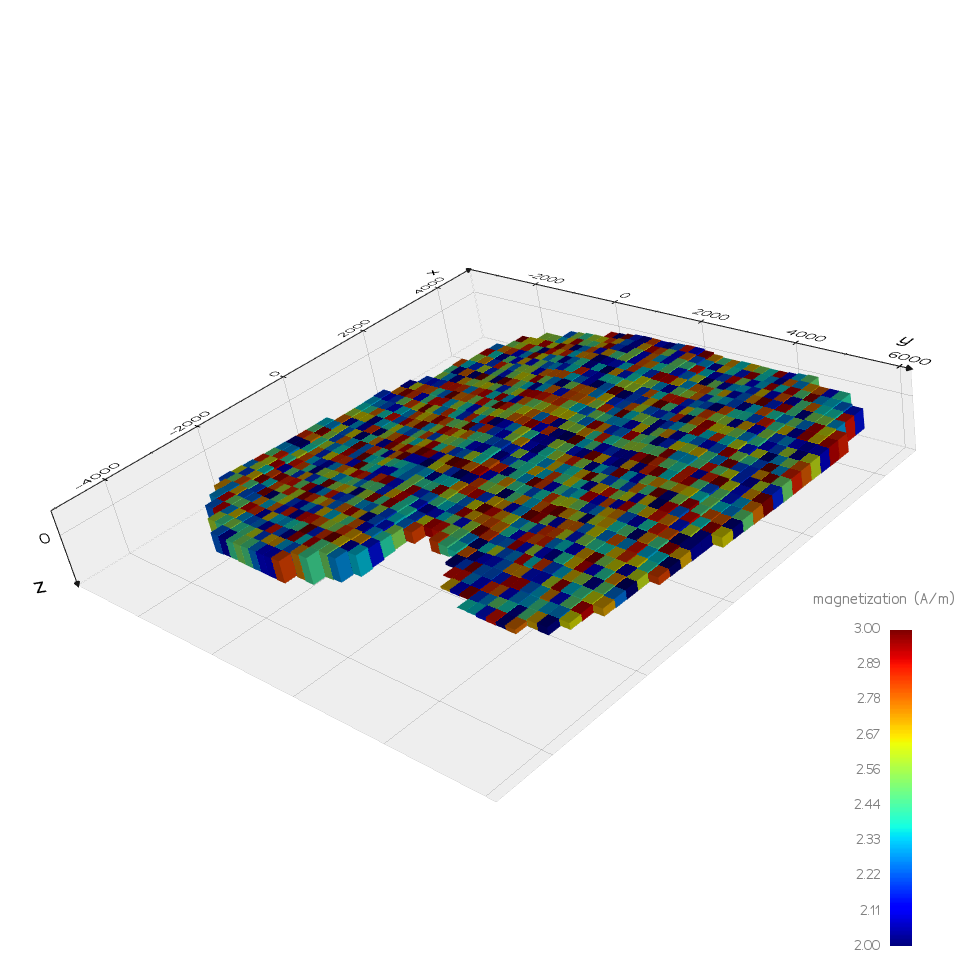
\includegraphics[width=0.8\textwidth]{figures/Figure2_2.png}
	\caption{%
		Simulated magnetic source formed by horizontally juxtaposed rectangular prisms. 
		The model have a pseudo-random total-magnetization intensity $\sigma$  
		varying uniformly from $2$ to $3$ A/m and a constant direction with inclination 
		$-10.2^{\circ}$ and declination $-19.8^{\circ}$.
	}
	\label{fig:Figure2}
\end{figure}

\begin{figure}
	\centering
	\noindent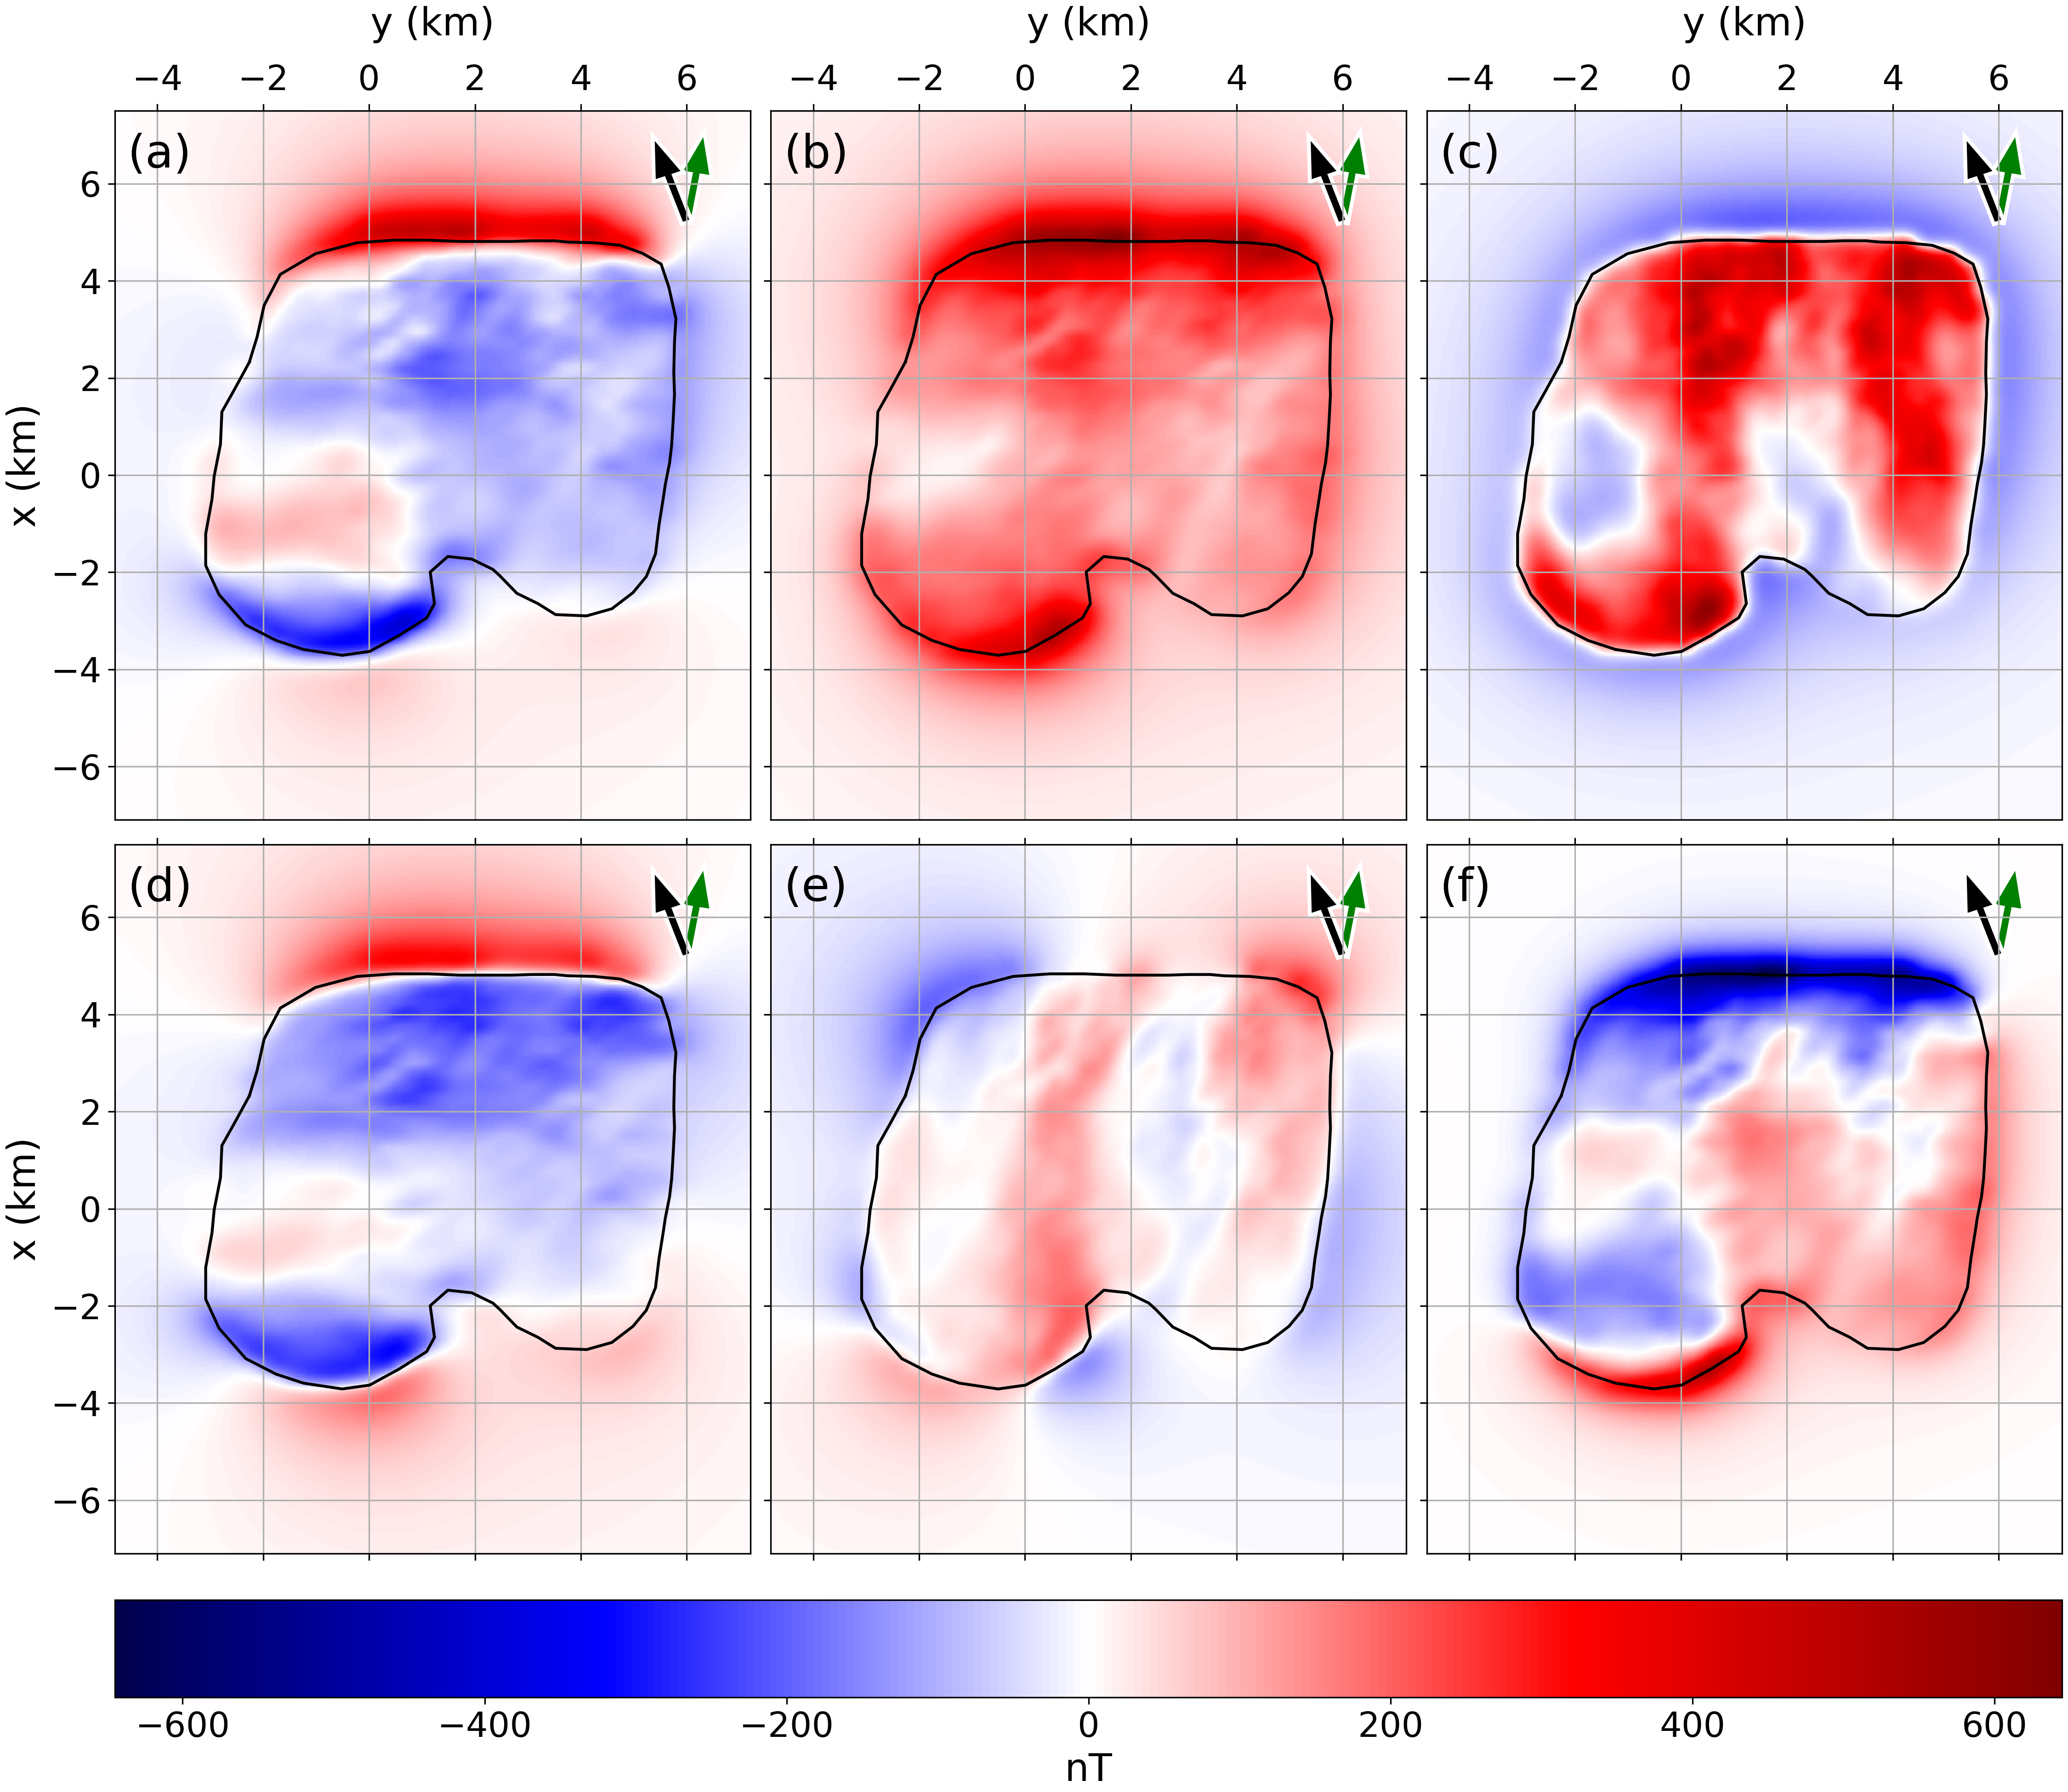
\includegraphics[width=0.8\textwidth]{figures/Figure2_3.png}
	\caption{%
		Potential fields due to the synthetic source (Fig. \ref{fig:Figure2}).
		(a) Approximated total-field anomaly, (b) amplitude of the magnetic induction field, 
		(c) RTP anomaly, (d), (e), (f) $x$, $y$ and $z$ components of the magnetic induction field,
		respectively. All values are in nT.	
		The black line represents the projection of the model on the $xy$ plane.
		The green and black arrows represent, respectively, the projections of the constant 
		main field and synthetic source (Fig. \ref{fig:Figure2}) magnetization directions onto the plane $xy$.
	}
	\label{fig:Figure3}
\end{figure}

\begin{figure}
	\centering
	\noindent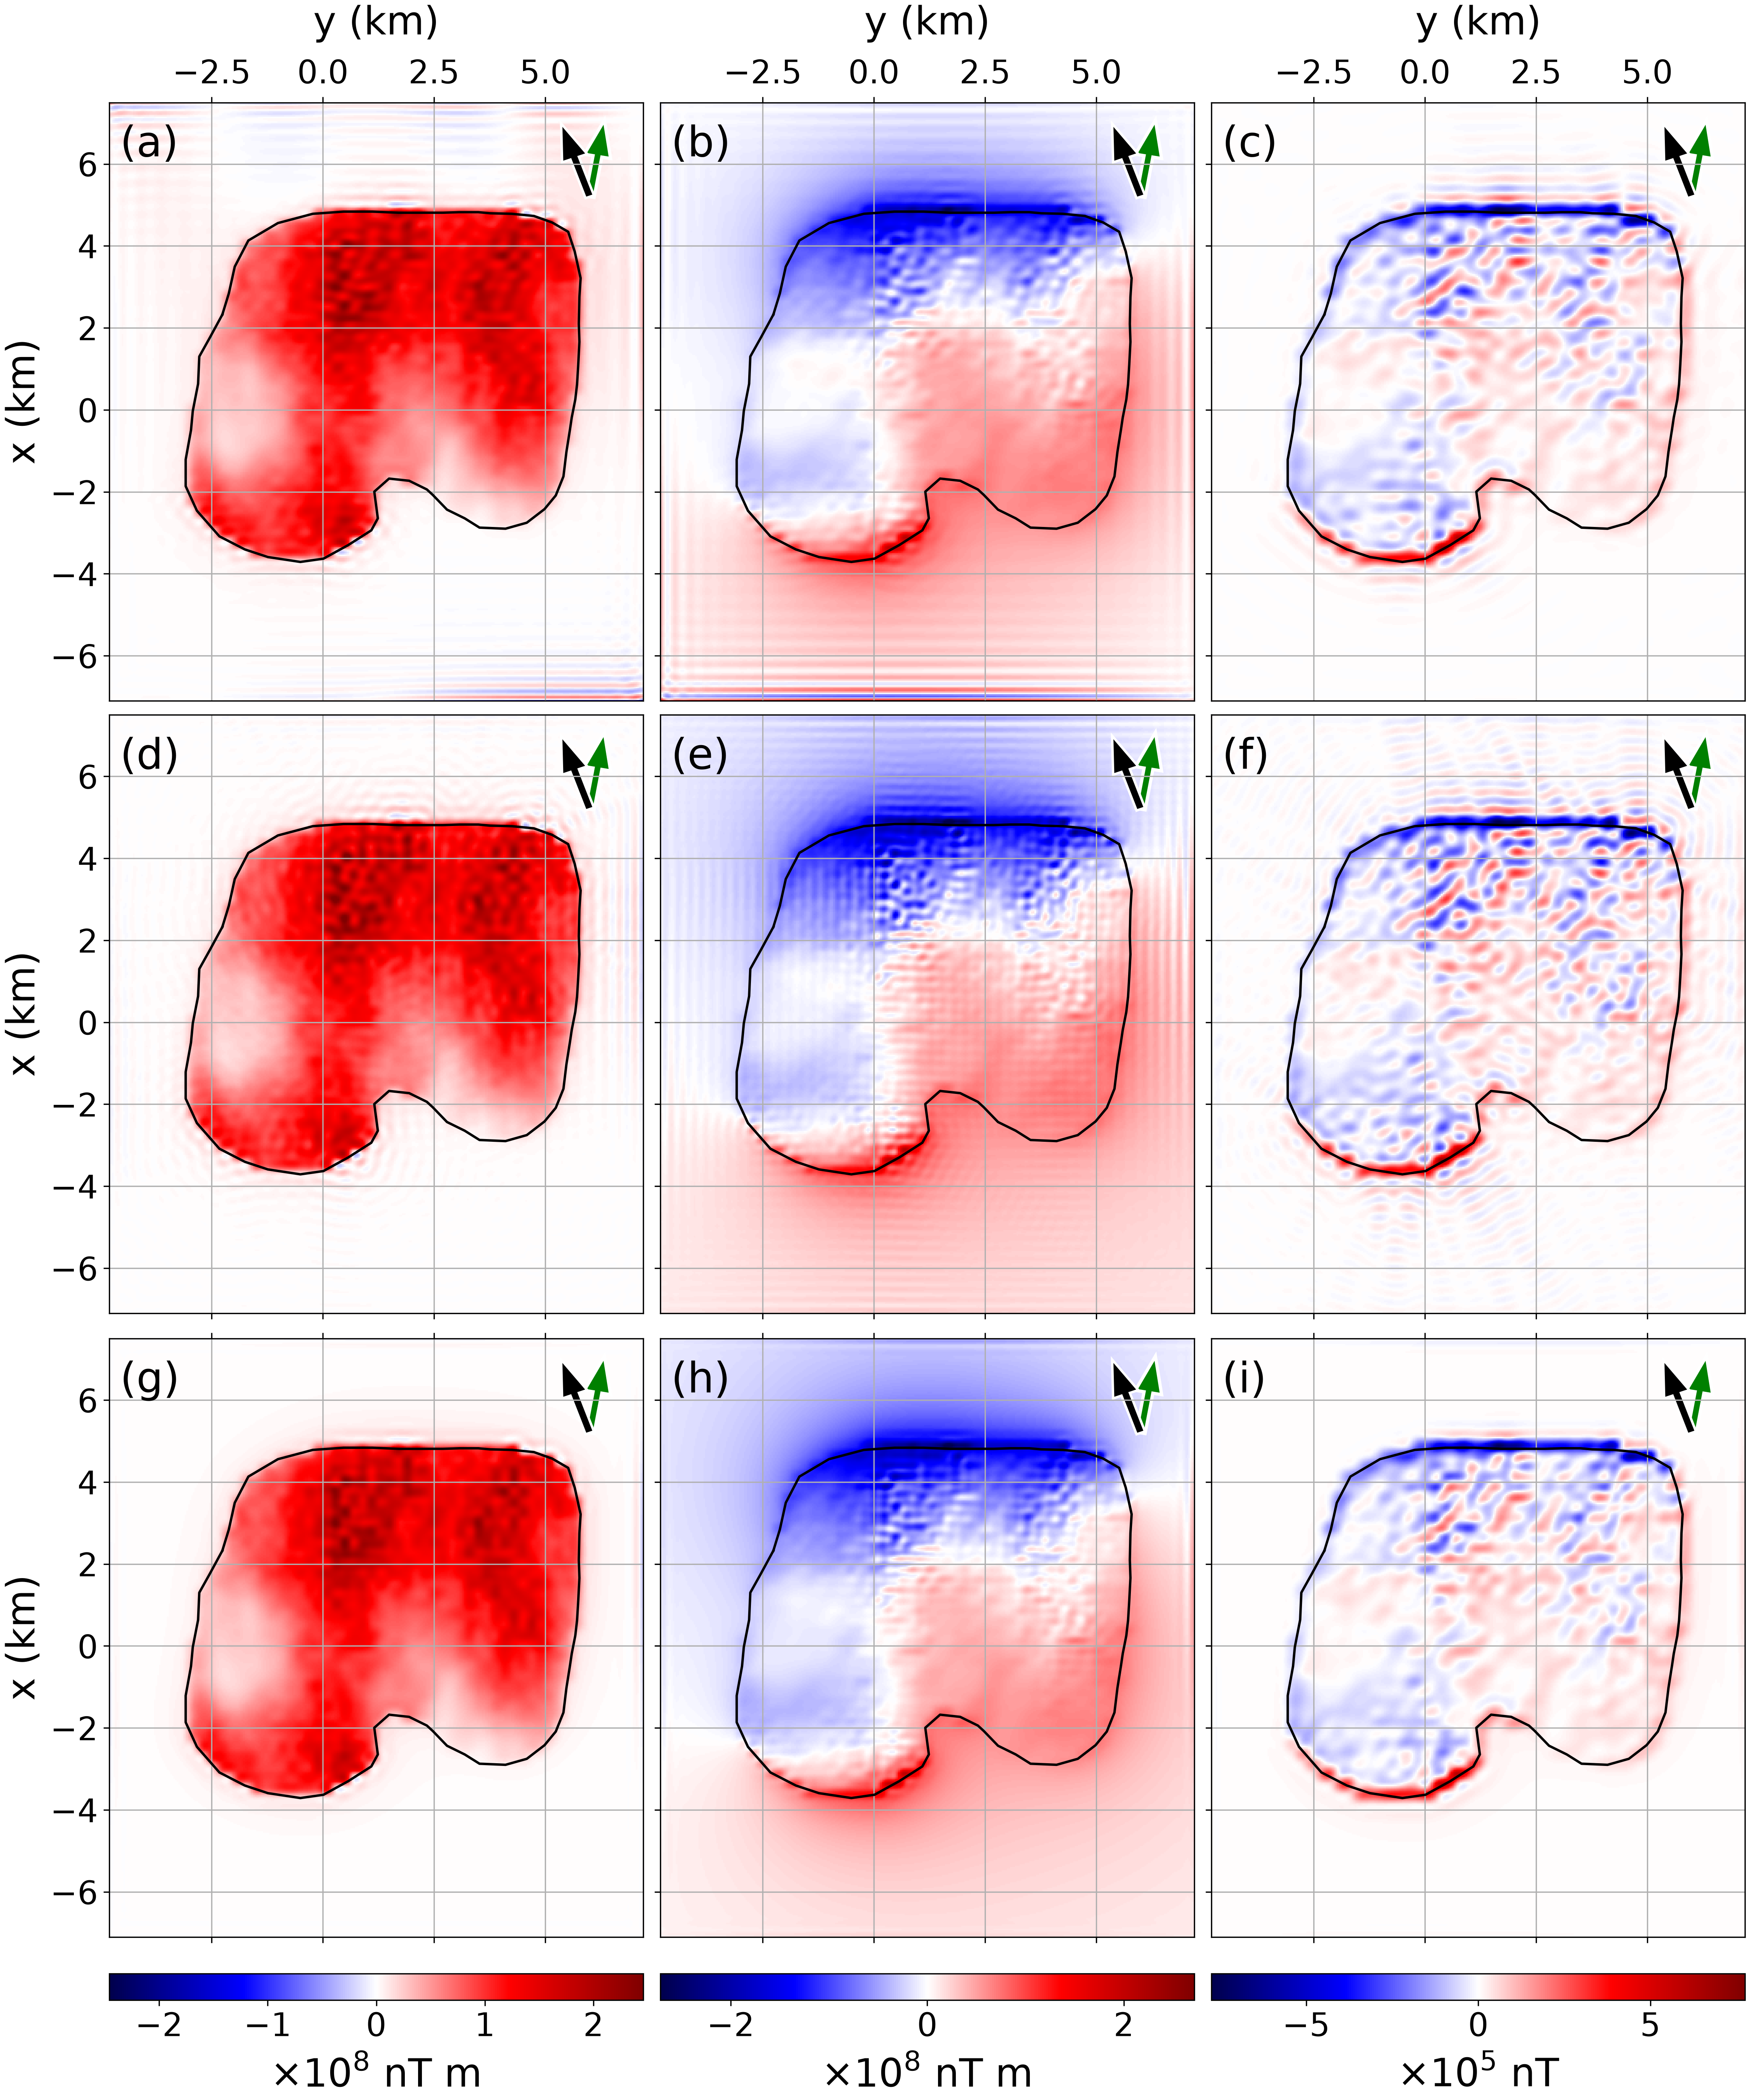
\includegraphics[width=0.8\textwidth]{figures/Figure2_4.png}
	\caption{%
		Estimated discrete layers.
		For all layers, we consider 
		$\alpha_{d} \equiv \alpha(1, \hat{\mathbf{u}}) \, \alpha(1, \hat{\mathbf{v}})$.
		The first, second and third columns contain the results obtained from each numerical test, 
		by using, respectively, $\alpha_{a} = \alpha_{d}$, 
		$\alpha_{a} = \left(\mathbf{k}^{\top} \hat{\mathbf{u}} \right) k$ and 
		$\alpha_{a} = \left(\mathbf{k}^{\top} \hat{\mathbf{u}} \right)$ (Eq. \ref{eq:p-Fourier}). 
		The first, second and third rows show, respectively, the layers estimated by following approaches 1--3.
		The black line represents the projection of the model on the $xy$ plane.
		The green and black arrows represent, respectively, the projections of the constant 
		main field and synthetic source (Fig. \ref{fig:Figure2}) magnetization directions onto the plane $xy$.
	}
	\label{fig:Figure4}
\end{figure}

\begin{figure}
	\centering
	\noindent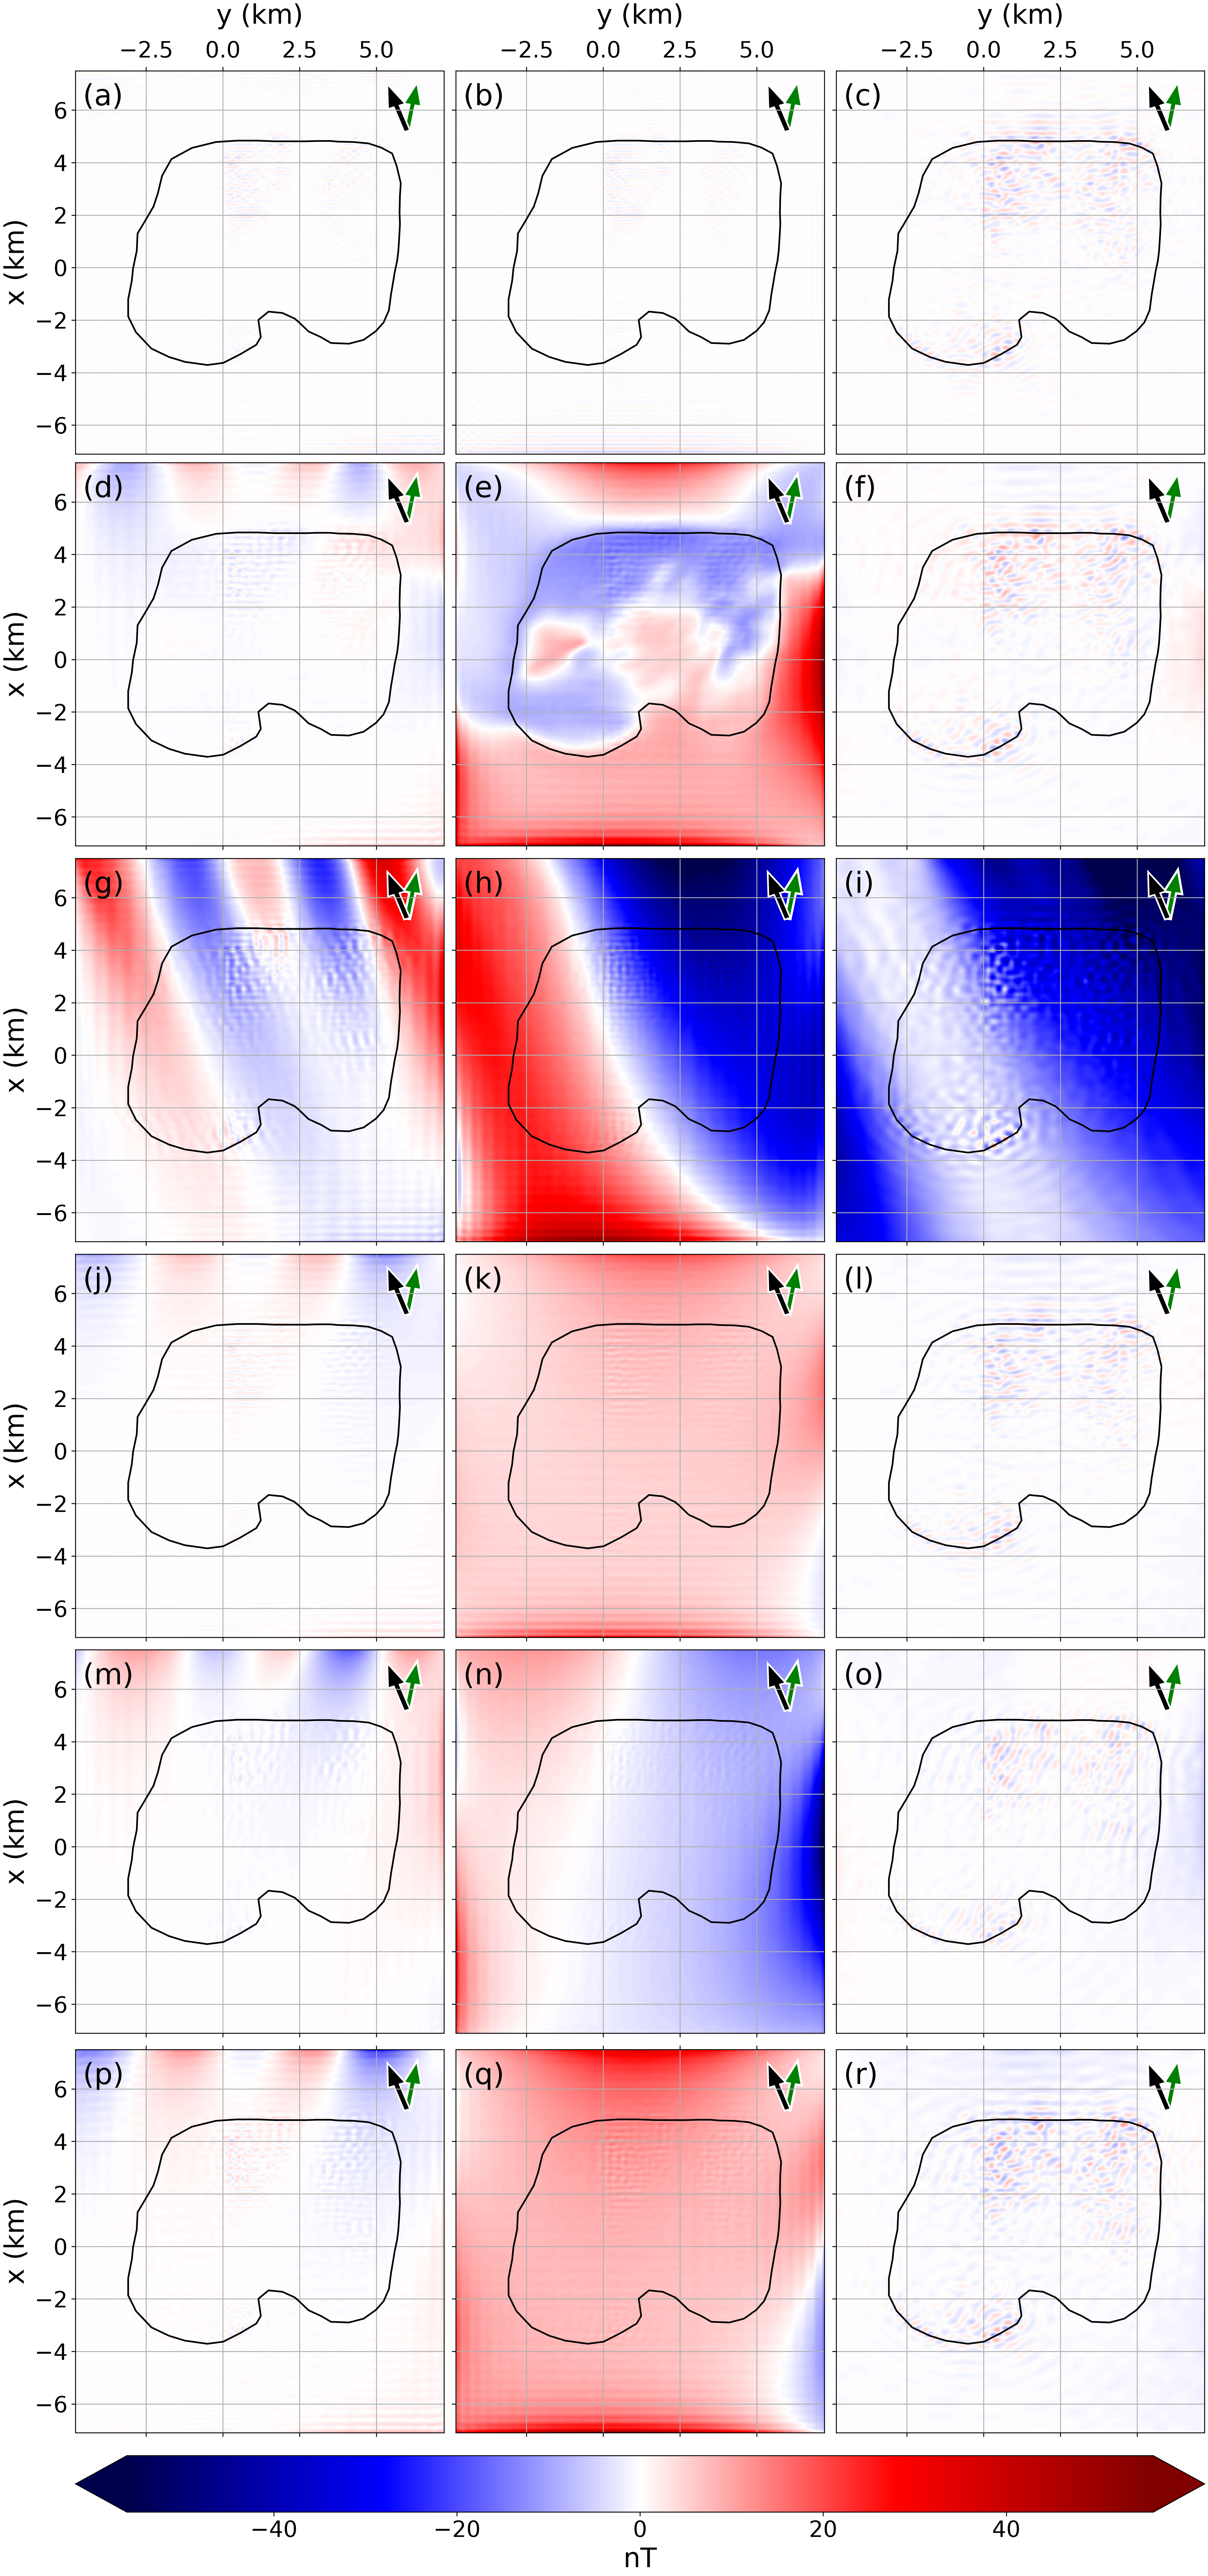
\includegraphics[width=0.65\textwidth]{figures/Figure2_5.png}
	\caption{%
		Residuals between the potential fields due to the synthetic source (Fig. \ref{fig:Figure2}) and
		those produced by the estimated layers shown in Figures \ref{fig:Figure4}a--c.
		The rows from top to bottom contain residuals of the approximated total-field anomaly,
		amplitude of magnetic induction field, RTP anomaly, $x$, $y$ and $z$ components of the magnetic induction field. 
		The columns from left to right contain the potential fields due to the layers shown, respectively, in Figures
		\ref{fig:Figure4}a--c. All values are in nT.
		The black line represents the projection of the model on the $xy$ plane.
		The green and black arrows represent, respectively, the projections of the constant 
		main field and synthetic source (Fig. \ref{fig:Figure2}) magnetization directions onto the plane $xy$.
	}
	\label{fig:Figure5}
\end{figure}
\section{Conclusions}
\label{sec:conclusions}

We have provided a theoretical foundation for several empirical approaches commonly 
associated with the equivalent-layer technique in geophysics. Our analysis clarifies why 
the widely used method has been so successful in applications such as the joint processing 
of gravity-gradient components, the conversion between gravity disturbances and gravity-gradient 
tensors, and the use of dipole layers for magnetic data processing and interpretation.

Synthetic tests show that discrete equivalent layers estimated by inversion of potential-field 
data closely approximate the closed-form expressions of continuous planar layers, 
whose existence is guaranteed by the planar equivalent-layer theorem. These findings 
confirm that planar equivalent layers are not merely mathematical abstractions but carry 
tangible physical significance rooted in boundary-value problems of potential theory.

Finally, we illustrated the use of an alternative dipole-based equivalent-layer approach 
in the interpretation of an airborne magnetic survey over the Registro do Araguaia alkaline 
complex in the Goiás Alkaline Province, Brazil. The results demonstrate that this formulation 
can recover the horizontal position of magnetic sources without requiring prior assumptions 
about their total magnetization.

\backmatter

%\bmhead{Supplementary information}
%
%If your article has accompanying supplementary file/s please state so here. 
%
%Authors reporting data from electrophoretic gels and blots should supply the full unprocessed scans for key as part of their Supplementary information. This may be requested by the editorial team/s if it is missing.
%
%Please refer to Journal-level guidance for any specific requirements.

\bmhead{Acknowledgements}
This study was financed by the Brazilian agencies Funda{\c c}{\~ a}o Carlos Chagas Filho de Amparo {\` a} Pesquisa do Estado do Rio de Janeiro (FAPERJ) 
(grant ids E-26 202.729/2018 and 26/202.582/2019) and Conselho Nacional de Desenvolvimento Cient{\' i}fico e Tecnol{\' o}gico (CNPq) (grant ids 315768/2020-7, 309624/2021-5 and 313493/2026-0). The authors thank the editors and reviewers who contributed to this work.

\section*{Declarations}

%Some journals require declarations to be submitted in a standardised format. Please check the Instructions for Authors of the journal to which you are submitting to see if you need to complete this section. If yes, your manuscript must contain the following sections under the heading `Declarations':

\begin{itemize}
%\item Funding
\item Conflict of interest/Competing interests: The authors declare no conflict of interest.
%\item Ethics approval and consent to participate: Not applicable.
%\item Consent for publication
%\item Data availability: Not applicable.
%\item Materials availability: Not applicable.
\item Code availability: The Python source code used to produce all results and figures presented in this study is
available at Zenodo \citep{dataset} under the MIT open-source license. This research made use of the following open-source scientific software: 
NumPy \citep{numpy} and SciPy \citep{scipy} for numerical computing and linear algebra, Matplotlib \citep{matplotlib} and Vedo \citep{vedo} for 
visualization, and gravmag \citep{gravmag} for potential field data processing and modeling. \textbf{The Dataset in \cite{dataset} will be made freely 
available at Zenodo upon publication. During the review process, we opted for sending the code directly for the editors and reviewers via submission 
system}.
%\item Author contribution
\end{itemize}

%\noindent
%If any of the sections are not relevant to your manuscript, please include the heading and write `Not applicable' for that section. 


%\begin{appendices}

%\section{Section title of first appendix}\label{secA1}
%
%An appendix contains supplementary information that is not an essential part of the text itself but which may be helpful in providing a more comprehensive understanding of the research problem or it is information that is too cumbersome to be included in the body of the paper.

%%=============================================%%
%% For submissions to Nature Portfolio Journals %%
%% please use the heading ``Extended Data''.   %%
%%=============================================%%

%%=============================================================%%
%% Sample for another appendix section			       %%
%%=============================================================%%

%% \section{Example of another appendix section}\label{secA2}%
%% Appendices may be used for helpful, supporting or essential material that would otherwise 
%% clutter, break up or be distracting to the text. Appendices can consist of sections, figures, 
%% tables and equations etc.

%\end{appendices}

%%===========================================================================================%%
%% If you are submitting to one of the Nature Portfolio journals, using the eJP submission   %%
%% system, please include the references within the manuscript file itself. You may do this  %%
%% by copying the reference list from your .bbl file, paste it into the main manuscript .tex %%
%% file, and delete the associated \verb+\bibliography+ commands.                            %%
%%===========================================================================================%%

\bibliography{references}% common bib file
%% if required, the content of .bbl file can be included here once bbl is generated
%%\input sn-article.bbl

\end{document}
